\documentclass[11pt,a4paper,]{article}
\usepackage{lmodern}

\usepackage{amssymb,amsmath}
\usepackage{ifxetex,ifluatex}
\usepackage{fixltx2e} % provides \textsubscript
\ifnum 0\ifxetex 1\fi\ifluatex 1\fi=0 % if pdftex
  \usepackage[T1]{fontenc}
  \usepackage[utf8]{inputenc}
\else % if luatex or xelatex
  \usepackage{unicode-math}
  \defaultfontfeatures{Ligatures=TeX,Scale=MatchLowercase}
\fi
% use upquote if available, for straight quotes in verbatim environments
\IfFileExists{upquote.sty}{\usepackage{upquote}}{}
% use microtype if available
\IfFileExists{microtype.sty}{%
\usepackage[]{microtype}
\UseMicrotypeSet[protrusion]{basicmath} % disable protrusion for tt fonts
}{}
\PassOptionsToPackage{hyphens}{url} % url is loaded by hyperref
\usepackage[unicode=true]{hyperref}
\hypersetup{
            pdftitle={Report on Happiness up to 2022},
            pdfborder={0 0 0},
            breaklinks=true}
\urlstyle{same}  % don't use monospace font for urls
\usepackage{geometry}
\geometry{a4paper, centering, text={16cm,25cm}}
\usepackage[style=apa,]{biblatex}
\addbibresource{references.bib}
\usepackage{longtable,booktabs}
% Fix footnotes in tables (requires footnote package)
\IfFileExists{footnote.sty}{\usepackage{footnote}\makesavenoteenv{long table}}{}
\usepackage{graphicx,grffile}
\makeatletter
\def\maxwidth{\ifdim\Gin@nat@width>\linewidth\linewidth\else\Gin@nat@width\fi}
\def\maxheight{\ifdim\Gin@nat@height>\textheight\textheight\else\Gin@nat@height\fi}
\makeatother
% Scale images if necessary, so that they will not overflow the page
% margins by default, and it is still possible to overwrite the defaults
% using explicit options in \includegraphics[width, height, ...]{}
\setkeys{Gin}{width=\maxwidth,height=\maxheight,keepaspectratio}
\IfFileExists{parskip.sty}{%
\usepackage{parskip}
}{% else
\setlength{\parindent}{0pt}
\setlength{\parskip}{6pt plus 2pt minus 1pt}
}
\setlength{\emergencystretch}{3em}  % prevent overfull lines
\providecommand{\tightlist}{%
  \setlength{\itemsep}{0pt}\setlength{\parskip}{0pt}}
\setcounter{secnumdepth}{5}

% set default figure placement to htbp
\makeatletter
\def\fps@figure{htbp}
\makeatother


\title{Report on Happiness up to 2022}

%% MONASH STUFF

%% CAPTIONS
\RequirePackage{caption}
\DeclareCaptionStyle{italic}[justification=centering]
 {labelfont={bf},textfont={it},labelsep=colon}
\captionsetup[figure]{style=italic,format=hang,singlelinecheck=true}
\captionsetup[table]{style=italic,format=hang,singlelinecheck=true}


%% FONT
\RequirePackage{bera}
\RequirePackage[charter,expert,sfscaled]{mathdesign}
\RequirePackage{fontawesome}

%% HEADERS AND FOOTERS
\RequirePackage{fancyhdr}
\pagestyle{fancy}
\rfoot{\Large\sffamily\raisebox{-0.1cm}{\textbf{\thepage}}}
\makeatletter
\lhead{\textsf{\expandafter{\@title}}}
\makeatother
\rhead{}
\cfoot{}
\setlength{\headheight}{15pt}
\renewcommand{\headrulewidth}{0.4pt}
\renewcommand{\footrulewidth}{0.4pt}
\fancypagestyle{plain}{%
\fancyhf{} % clear all header and footer fields
\fancyfoot[C]{\sffamily\thepage} % except the center
\renewcommand{\headrulewidth}{0pt}
\renewcommand{\footrulewidth}{0pt}}

%% MATHS
\RequirePackage{bm,amsmath}
\allowdisplaybreaks

%% GRAPHICS
\RequirePackage{graphicx}
\setcounter{topnumber}{2}
\setcounter{bottomnumber}{2}
\setcounter{totalnumber}{4}
\renewcommand{\topfraction}{0.85}
\renewcommand{\bottomfraction}{0.85}
\renewcommand{\textfraction}{0.15}
\renewcommand{\floatpagefraction}{0.8}


%\RequirePackage[section]{placeins}

%% SECTION TITLES


%% SECTION TITLES
\RequirePackage[compact,sf,bf]{titlesec}
\titleformat*{\section}{\Large\sf\bfseries\color[rgb]{0.7,0,0}}
\titleformat*{\subsection}{\large\sf\bfseries\color[rgb]{0.7,0,0}}
\titleformat*{\subsubsection}{\sf\bfseries\color[rgb]{0.7,0,0}}
\titlespacing{\section}{0pt}{2ex}{.5ex}
\titlespacing{\subsection}{0pt}{1.5ex}{0ex}
\titlespacing{\subsubsection}{0pt}{.5ex}{0ex}


%% TITLE PAGE
\def\Date{\number\day}
\def\Month{\ifcase\month\or
 January\or February\or March\or April\or May\or June\or
 July\or August\or September\or October\or November\or December\fi}
\def\Year{\number\year}

%% LINE AND PAGE BREAKING
\sloppy
\clubpenalty = 10000
\widowpenalty = 10000
\brokenpenalty = 10000
\RequirePackage{microtype}

%% PARAGRAPH BREAKS
\setlength{\parskip}{1.4ex}
\setlength{\parindent}{0em}

%% HYPERLINKS
\RequirePackage{xcolor} % Needed for links
\definecolor{darkblue}{rgb}{0,0,.6}
\RequirePackage{url}

\makeatletter
\@ifpackageloaded{hyperref}{}{\RequirePackage{hyperref}}
\makeatother
\hypersetup{
     citecolor=0 0 0,
     breaklinks=true,
     bookmarksopen=true,
     bookmarksnumbered=true,
     linkcolor=darkblue,
     urlcolor=blue,
     citecolor=darkblue,
     colorlinks=true}

\usepackage[showonlyrefs]{mathtools}
\usepackage[no-weekday]{eukdate}

%% BIBLIOGRAPHY

\makeatletter
\@ifpackageloaded{biblatex}{}{\usepackage[style=authoryear-comp, backend=biber, natbib=true]{biblatex}}
\makeatother
\ExecuteBibliographyOptions{bibencoding=utf8,minnames=1,maxnames=3, maxbibnames=99,dashed=false,terseinits=true,giveninits=true,uniquename=false,uniquelist=false,doi=false, isbn=false,url=true,sortcites=false}

\DeclareFieldFormat{url}{\texttt{\url{#1}}}
\DeclareFieldFormat[article]{pages}{#1}
\DeclareFieldFormat[inproceedings]{pages}{\lowercase{pp.}#1}
\DeclareFieldFormat[incollection]{pages}{\lowercase{pp.}#1}
\DeclareFieldFormat[article]{volume}{\mkbibbold{#1}}
\DeclareFieldFormat[article]{number}{\mkbibparens{#1}}
\DeclareFieldFormat[article]{title}{\MakeCapital{#1}}
\DeclareFieldFormat[article]{url}{}
%\DeclareFieldFormat[book]{url}{}
%\DeclareFieldFormat[inbook]{url}{}
%\DeclareFieldFormat[incollection]{url}{}
%\DeclareFieldFormat[inproceedings]{url}{}
\DeclareFieldFormat[inproceedings]{title}{#1}
\DeclareFieldFormat{shorthandwidth}{#1}
%\DeclareFieldFormat{extrayear}{}
% No dot before number of articles
\usepackage{xpatch}
\xpatchbibmacro{volume+number+eid}{\setunit*{\adddot}}{}{}{}
% Remove In: for an article.
\renewbibmacro{in:}{%
  \ifentrytype{article}{}{%
  \printtext{\bibstring{in}\intitlepunct}}}

\AtEveryBibitem{\clearfield{month}}
\AtEveryCitekey{\clearfield{month}}

\makeatletter
\DeclareDelimFormat[cbx@textcite]{nameyeardelim}{\addspace}
\makeatother

\author{\sf{\Large\textbf{(Elvis) Zhixiang Yang}\\\large EBS Honours Student\\[0.5cm]}{\Large\textbf{Yiqi Wang}\\\large Master of BA Student\\[0.5cm]}{\Large\textbf{Xintong You}\\\large Master of BA Student\\[0.5cm]}}

\date{\sf\Date~\Month~\Year}
\makeatletter
\lfoot{\sf Yang, Wang, You: \@date}
\makeatother


%%%% PAGE STYLE FOR FRONT PAGE OF REPORTS

\makeatletter
\def\organization#1{\gdef\@organization{#1}}
\def\telephone#1{\gdef\@telephone{#1}}
\def\email#1{\gdef\@email{#1}}
\makeatother
  \organization{Group 07 ETC5513}

  \def\name{Department of\newline Econometrics \&\newline Business Statistics}

  \telephone{(03) 9905 2478}

  \email{BusEco-Econometrics@monash.edu}

\def\webaddress{\url{http://buseco.monash.edu/ebs/consulting/}}
\def\abn{12 377 614 012}
\def\extraspace{\vspace*{1.6cm}}
\makeatletter
\def\contactdetails{\faicon{phone} & \@telephone \\
                    \faicon{envelope} & \@email}
\makeatother

\usepackage[absolute,overlay]{textpos}
\setlength{\TPHorizModule}{1cm}
\setlength{\TPVertModule}{1cm}

%%%% FRONT PAGE OF REPORTS

\def\reporttype{Report for}

\long\def\front#1#2#3{
\newpage
\begin{textblock}{7}(12.7,28.2)\hfill

\includegraphics[height=0.6cm]{AACSB}~~~

\includegraphics[height=0.6cm]{EQUIS}~~~

\includegraphics[height=0.6cm]{AMBA}
\end{textblock}
\begin{singlespacing}
\thispagestyle{empty}
\vspace*{-1.4cm}
\hspace*{-1.4cm}
\hbox to 16cm{
  \hbox to 6.5cm{\vbox to 14cm{\vbox to 25cm{
    
\includegraphics[width=6cm]{monash2}
    \vfill
    
\includegraphics[width=3.5cm]{MBSportrait}
    \vspace{0.4cm}
    \par
    \parbox{6.3cm}{\raggedright
      \sf\color[rgb]{0.00,0.00,0.70}
      {\large\textbf{\name}}\par
      \vspace{.7cm}
      \tabcolsep=0.12cm\sf\small
      \begin{tabular}{@{}ll@{}}\contactdetails
      \end{tabular}
      \vspace*{0.3cm}\par
      ABN: \abn\par
    }
  }\vss}\hss}
  \hspace*{0.2cm}
  \hbox to 1cm{\vbox to 14cm{\rule{1pt}{26.8cm}\vss}\hss\hfill}
  \hbox to 10cm{\vbox to 14cm{\vbox to 25cm{
      \vspace*{3cm}\sf\raggedright
      \parbox{11cm}{\sf\raggedright\baselineskip=1.2cm
         \fontsize{24.88}{30}\color[rgb]{0.70,0.00,0.00}\sf\textbf{#1}}
      \par
      \vfill
      \large
      \vbox{\parskip=0.8cm #2}\par
      \vspace*{2cm}\par
      \reporttype\\[0.3cm]
      \hbox{#3}%\\[2cm]\
      \vspace*{1cm}
      {\large\sf\textbf{\Date~\Month~\Year}}
   }\vss}
  }}
\end{singlespacing}
\newpage
}

\makeatletter
\def\titlepage{\front{\expandafter{\@title}}{\@author}{\@organization}}
\makeatother

\usepackage{setspace}
\setstretch{1.5}

%% Any special functions or other packages can be loaded here.
\usepackage[normalem]{ulem}
\usepackage{float}
\useunder{\uline}{\ul}{}
\usepackage{float}
\usepackage{amsmath}
\usepackage{booktabs}
\usepackage{longtable}
\usepackage{array}
\usepackage{multirow}
\usepackage{wrapfig}
\usepackage{colortbl}
\usepackage{pdflscape}
\usepackage{tabu}
\usepackage{threeparttable}
\usepackage{threeparttablex}
\usepackage[normalem]{ulem}
\usepackage{makecell}
\usepackage{xcolor}


\begin{document}
\titlepage

{
\setcounter{tocdepth}{2}
\tableofcontents
}
\clearpage

\hypertarget{introduction}{%
\section{Introduction}\label{introduction}}

\textcite{rojas2010} stated that many factors might contribute to the happiness score. They also mentioned that the conceptions of happiness differ not only across people, but also across the culture and region etc. If we want to improve the happiness, we cannot stimulate all relevant variables. Thus, an analysis about the world happiness report will help to figure out several common key variables that influence the happiness of human beings. Then, we can try to improve the at a worldwide level, especially after the pandemic.

Apart from this, \textcite{helliwell2021world} stated that the global pandemic has significantly influenced the happiness of people in different regions. Considering the pandemic, we will also analyse the impacts of COVID-19 to the happiness score for top-ranking countries and the variable relationships after the pandemic happened.

In the modelling part, we will provide a detailed analysis of the data fits in various models. After obtaining two most important variables, we will add another two new relevant variables to build up a multivariate linear regression model with data from 2016 to 2020.

However, it is common to have heteroskedasticity problem in the model. Besides, some variables are not collected after year 2020, leading the model to be not perfect. Critical analysis will be conducted in the end, supported by residual diagnostic.

\hypertarget{research-questions}{%
\section{Research Questions}\label{research-questions}}

The report will be divided into different sections to explore following research questions:

\begin{itemize}
\item
  The influences of COVID-19 on the world happiness score and the correlations between happiness in 2021.
\item
  The changes of happiness between 2015 and 2022 in different regions.
\item
  The impact of economic situation and health status on happiness.
\item
  The important variable in explaining happiness scores via different models and discover their marginal effects in a linear model.
\end{itemize}

\hypertarget{data}{%
\section{Data}\label{data}}

\hypertarget{description}{%
\subsection{Description}\label{description}}

Our data comes from Kaggle, which is a report of the World Happiness. In the eight datasets, the variables explaining the happiness score including Economy(measured in GDP per capita), Health status, Freedom, Generosity are consistent each year. Nevertheless, after year 2020, few new variables have been added and there are few changes with the existing variables. The happiness score is ranked from the highest to the lowest one and gained via an anonymous worldwide survey across different countries around the world.

Apart from our existing data, we will also join two new datasets in the modelling part gained from the World Bank Data due to the potential issues in our existing dataset. More information will be discussed in the multivariate linear model part.

\hypertarget{pre-processing.}{%
\subsection{Pre-processing.}\label{pre-processing.}}

The data gained from Kaggle is not clean. In this report, we tried to combine all the historical data with common factors, which are Economy, Health, Freedom, Generosity each year and drop the NA values. However, for specific yearly analysis after 2020, we decide to keep all the new variable in explaining the happiness score.

In addition, two variable related to Consumer Price Index and Populations from the World Bank data will be joined across different countries in each year when we trying to build up our multivariate linear model.

\hypertarget{exploratory-data-analysis-world-happiness-from-2015-to-2022}{%
\section{Exploratory Data Analysis (World Happiness from 2015 to 2022)}\label{exploratory-data-analysis-world-happiness-from-2015-to-2022}}

In this part, we will investigate the trends of happiness score represented by region between 2015 and 2022. After this, we will analyse the impacts of annual health and economic status on happiness score.

Combined with my research questions, I consolidate all the datasets for each year between 2015 to 2022 into a new dataset, and then tease out the variables to use, which are year, region, happiness score, economy, and health.

\hypertarget{the-development-of-the-world-happiness}{%
\subsection{The development of the World Happiness}\label{the-development-of-the-world-happiness}}

\textcite{helliwell2012state} stated that with the continuous progress of human society, the happiness index has become an important indicator for measuring the living standards across regions. Meanwhile, people have also realized the importance to apply the happiness index in macroeconomic analysis. In the real world, the happiness index is related to many factors, it will also affect nearly all aspects of human activities. Thus, we will start with two research questions to explore the happiness index of the world.

\hypertarget{research-questions-1}{%
\subsection{Research questions}\label{research-questions-1}}

\begin{itemize}
\item
  How will happiness trends change between 2015 to 2022 in different regions?
\item
  What is the relationship impacts of economic situation and health status to the happiness score?
\end{itemize}

\hypertarget{the-trends-in-happiness-2015-2022}{%
\subsection{The trends in happiness 2015-2022}\label{the-trends-in-happiness-2015-2022}}

\begin{figure}
\centering
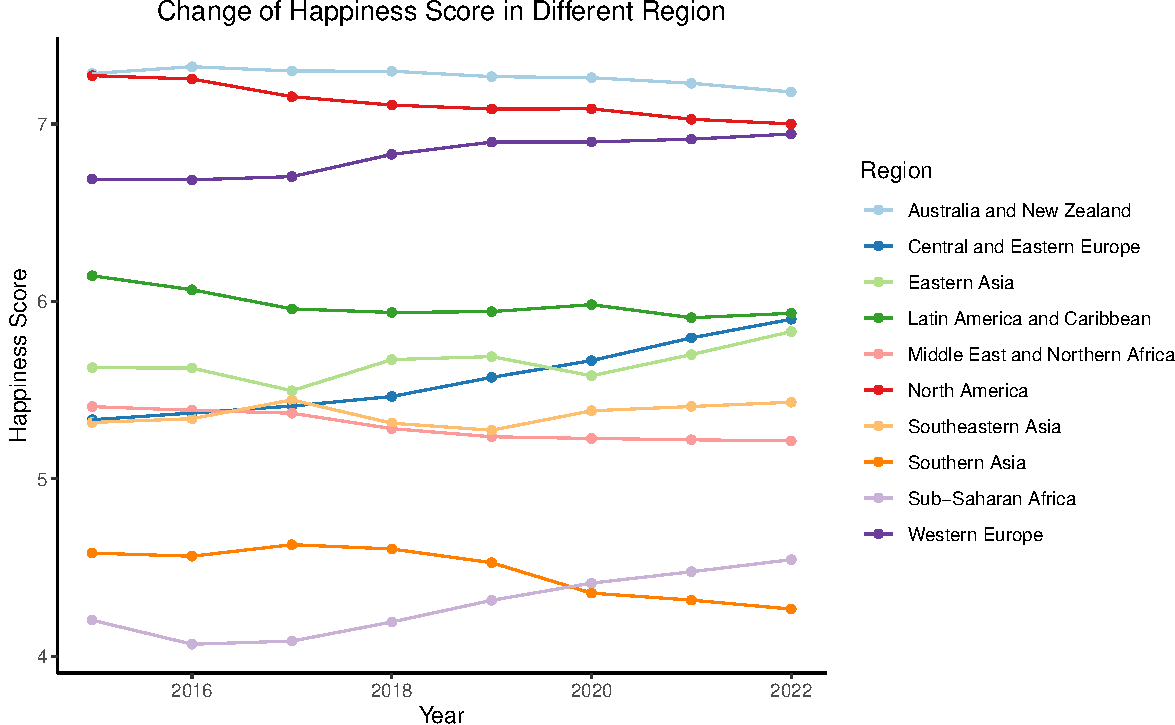
\includegraphics{Assignment4_files/figure-latex/trends-1.pdf}
\caption{\label{fig:trends}Change of Happiness Score in Different Region}
\end{figure}

From the Figure \ref{fig:trends}, we can see that the trend in all regions can be divided into three different levels of happiness score.

We can see from the plot that South Asia and Sub-Saharan Africa remained at low level for the past few years. While Southern Asia countries started declining in 2017, Sub-Saharan Africa's happiness began to increase year by year after reaching the trough in 2016. In addition, the declining trend of happiness for people in Southeastern Asia may due to the population booming in these years.

Moreover, the three regions had a relatively high scores are: Australia and New Zealand, North America, and Western Europe. We can see people living in these developed area feels happier than others, which may be due to the good social welfare, less stress and better working environment. Nevertheless, an interesting point to notice is that even there are many modern countries in Eastern Asia, people didn't really feel happy in the past few years. This may due to the living condition and working stresses are high from these Eastern Asian countries.

Then, the remaining regions are all centered in middle level. Among these regions, Central and Eastern Europe is the only region have an obvious increasing trend over the years, while the rest of the region is in a state of slightly fluctuating but generally stable trends.

Overall, we conclude that for those regions with relatively better economic situation and social welfare would generally lead to a higher happiness scores with less fluctuations than those regions with poor economic situation.

\hypertarget{the-relationship-between-economic-situation-and-health-status-with-the-happiness-in-2015-2022}{%
\subsection{The relationship between economic situation and health status with the happiness in 2015-2022}\label{the-relationship-between-economic-situation-and-health-status-with-the-happiness-in-2015-2022}}

People's understanding of happiness is inseparable from their own living conditions. In this section, we will also explore the relationship between happiness and economic and health status.

From the figure \ref{fig:VS}, we can find that there is a positive correlation between economic status, health status and happiness score from 2015 to 2022, which is make sense that a better the economic status and health status will make people happier.

There is an overall trend from 2015 to 2022 that the correlation of health and happiness is increasing over the years. Nevertheless, the correlation of economic situation is decreasing. This may due to the situation that people have better economic situation nowadays and they pay more attention on their health status.

From 2017 to 2018, the average influences of economic on happiness score increased slightly, while the influence of health on happiness score decreased slightly during this period.

On the other hand, from 2019 to 2022, the influence of the economic status on the happiness score is getting lower while the influence of the health on the happiness score has increased significantly especially after 2020, which maybe due to the pandemic that people care more about their health status.

\begin{figure}
\centering
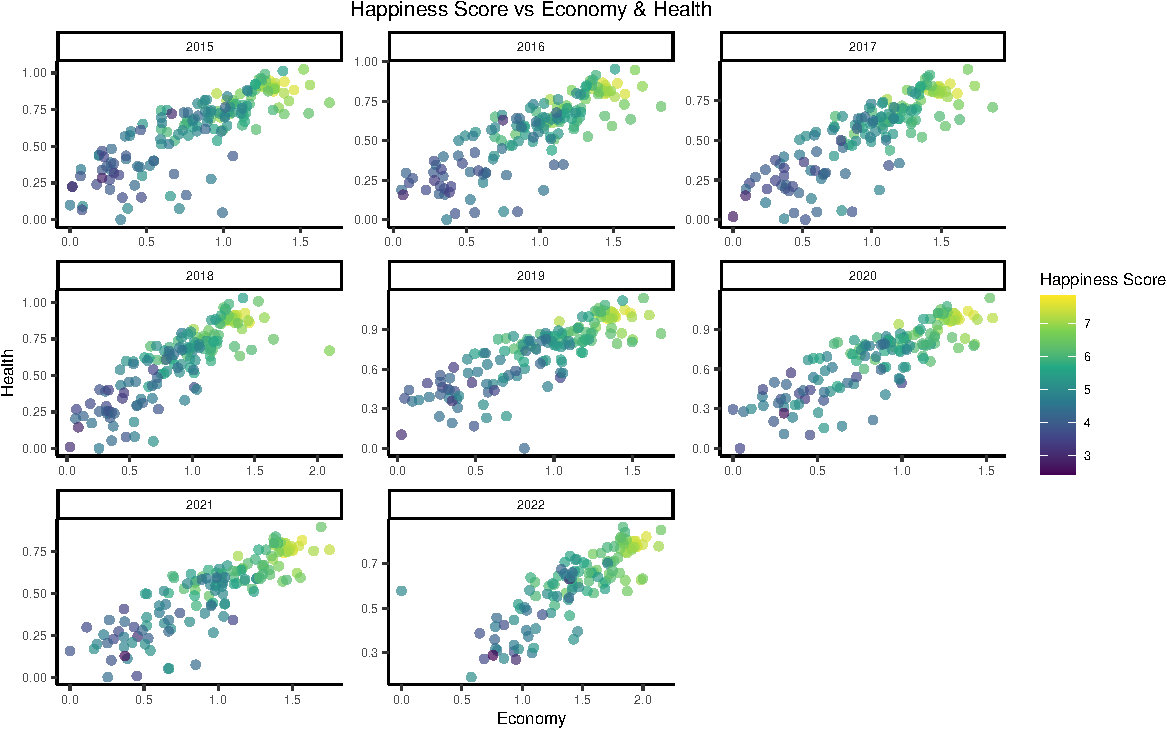
\includegraphics{Assignment4_files/figure-latex/VS-1.pdf}
\caption{\label{fig:VS}Happiness Score vs Economy \& Health}
\end{figure}

\newpage

\begin{table}
\centering
\begin{tabular}{|c|c|c|c|}
\hline
\textbf{Year} & \textbf{Intercept} & \textbf{Economy} & \textbf{Health} \\
\hline
2015          & 3.250              & 1.616            & 1.203           \\
2016          & 2.980              & 1.516            & 1.662           \\
2017          & 2.968              & 1.504            & 1.632           \\
2018          & 3.085              & 1.511            & 1.565           \\
2019          & 2.892              & 1.359            & 1.775           \\
2020          & 3.117              & 1.305            & 1.791           \\
2021          & 3.298              & 1.316            & 1.854           \\
2022          & 2.370              & 1.406            & 2.085           \\
\hline
\end{tabular}
\caption{Simple linear relationship between economic status and health status with happiness score each year: 3-digits}
\label{tab:table}
\end{table}

We also conducted an simple regression analysis. From the Table \ref{tab:table}, we can see the impact of economic situation on the slope decreased very slowly from 1.616 to 1.406 over the years. On the contrary, the influence of health on happiness score changed a lot with the slope increased from 1.2 to 2.08. Through this simple linear regression analysis, we can also see that people gradually focus on their health status nowadays.

\newpage

\hypertarget{exploratory-data-analysis-pandemic-influences}{%
\section{Exploratory data analysis (Pandemic Influences)}\label{exploratory-data-analysis-pandemic-influences}}

\hypertarget{introduction-1}{%
\subsection{Introduction}\label{introduction-1}}

According to \textcite{helliwell2021world}, economic situation, people's health and freedom have been severely affected across different countries since the outbreak of COVID-19 in 2020, which will directly impact the world.

In the following research, the top 10 happiest countries in the world and their regions will be explored. Then, factors associated with the happiness score will be explored by analyzing the relation between happiness score and six selected indicators in 2021.

\hypertarget{what-are-the-countries-which-ranks-top-10-in-happiness-score-since-the-covid-19-outbreak}{%
\subsection{What are the countries which ranks top 10 in happiness score since the COVID-19 outbreak?}\label{what-are-the-countries-which-ranks-top-10-in-happiness-score-since-the-covid-19-outbreak}}

\begin{figure}
\centering
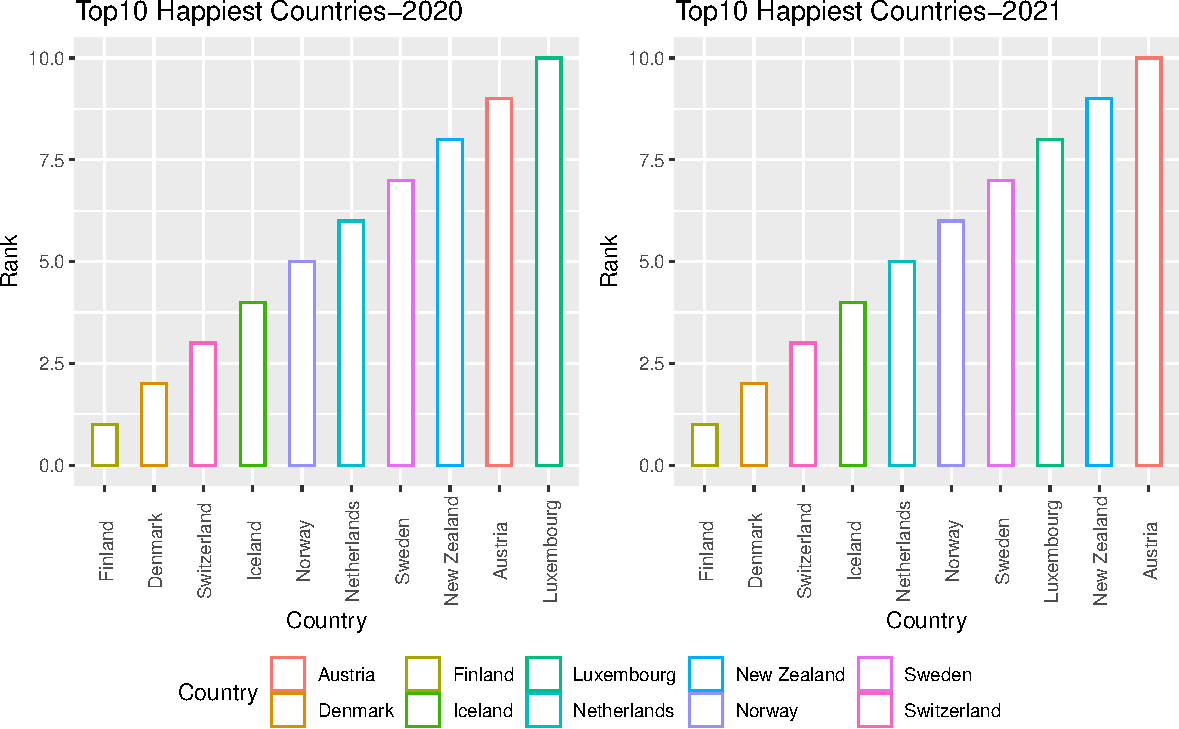
\includegraphics{Assignment4_files/figure-latex/top10-1.pdf}
\caption{\label{fig:top10}The top 10 countries in happiness score since COVID-19}
\end{figure}

In the Figure \ref{fig:top10}, the top 10 countries in the World Happiness have not changed since 2020 despite the impact of COVID-19, while their ranks have changed slightly.

In addition, Finland has been the happiest country for two consecutive years in 2020 and 2021. We believe this is mainly due to the fact that Finland has a well structured social welfare and health care system \autocite{lappi2006finland}.

\hypertarget{the-distribution-of-the-top-10-countries-on-the-world-map-in-2021}{%
\subsection{The distribution of the top 10 countries on the world map in 2021}\label{the-distribution-of-the-top-10-countries-on-the-world-map-in-2021}}

\begin{figure}
\centering
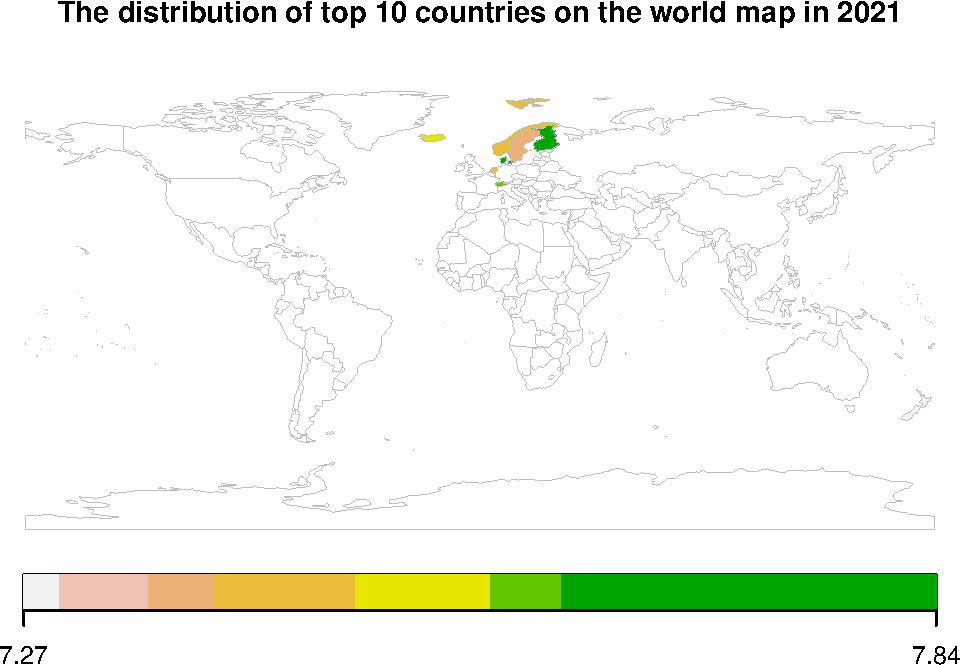
\includegraphics{Assignment4_files/figure-latex/top10map-1.pdf}
\caption{\label{fig:top10map}The distribution of top 10 countries on the world map in 2021}
\end{figure}

According to the Figure \ref{fig:top10map}, these countries are mainly northern and western European countries.Obviously, they are all developed countries which have a technologically advanced infrastructure and their economy is highly developed.

So besides high economy, what are the other indicators that can affect happiness score?

\hypertarget{relation-between-happiness-score-and-other-indicators-in-2021}{%
\subsection{Relation between Happiness score and other indicators in 2021}\label{relation-between-happiness-score-and-other-indicators-in-2021}}

\begin{figure}
\centering
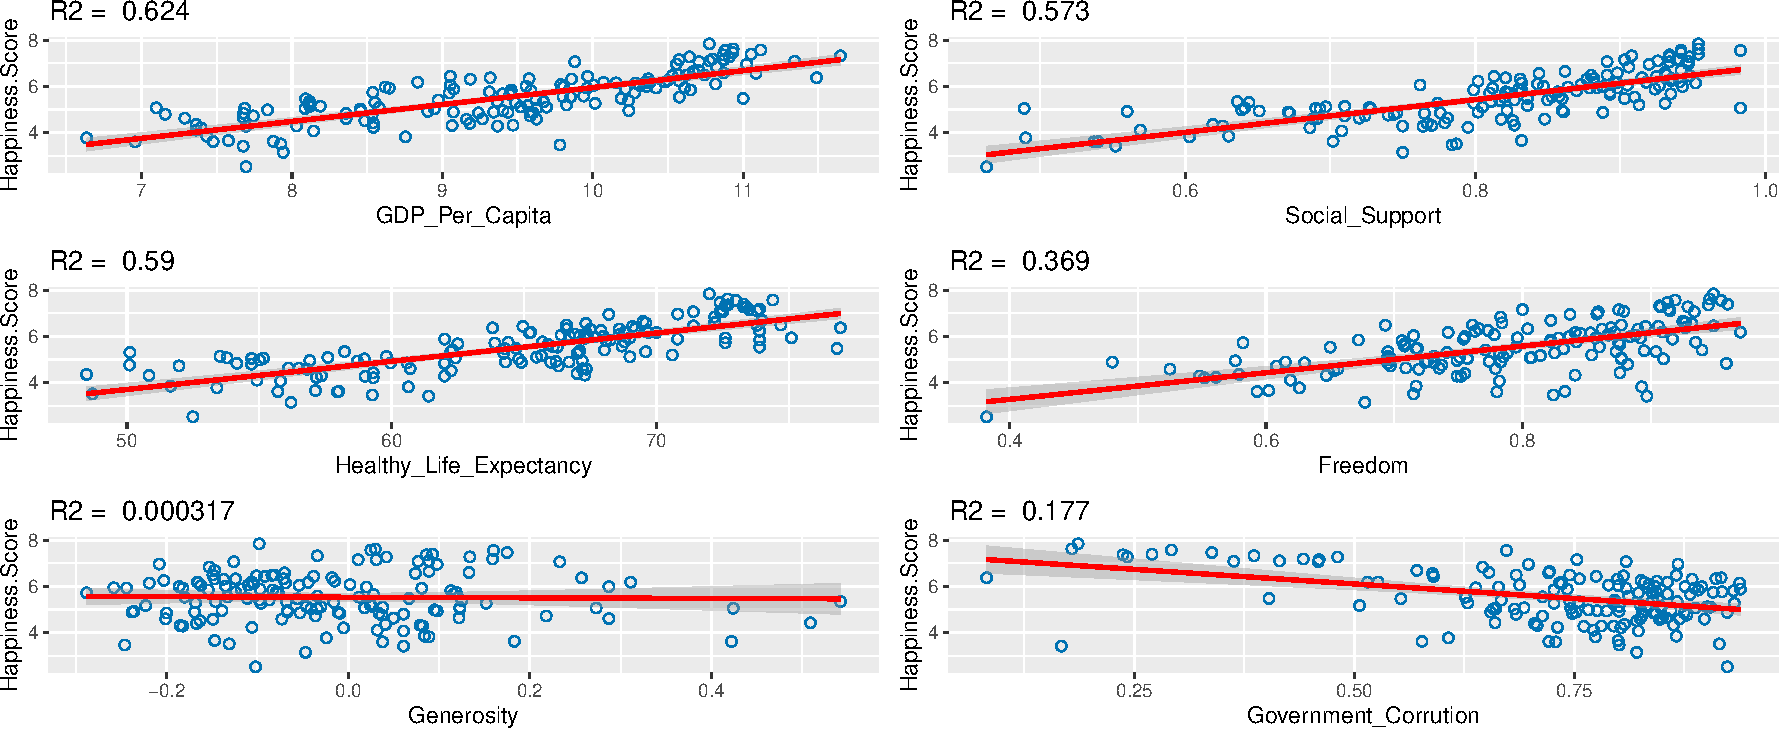
\includegraphics{Assignment4_files/figure-latex/relation-1.pdf}
\caption{\label{fig:relation}Relation between Happiness score and 6 indicators in 2021}
\end{figure}

The 6 linear graphs in Figure \ref{fig:relation} demonstrate the relationships between the happiness and 6 attributes of the countries in 2021. R-squared (\(R^2\)) represents the proportion of the variance for happiness that's explained by an independent variable in the regression model. For example, in the graph on the upper left, its R-squared is 0.624, indicating that there are 62.4\% of their happiness scores can be explained by their GDP.

Therefore, we can see that both social support and health life expectancy explain happiness in a relatively high proportion which is 57.3\% and 59\% respectively. While freedom, generosity and trust in government corruption are not good in explaining happiness score.

To summarize, in this part we found the world's top 10 happiest countries are mainly concentrated in Northern and Western Europe in 2020 and 2021, which have high economic level and GDP. From the data of the world, the variables highly related to happiness are \textbf{GDP, social support and health life expectancy}.

\clearpage

\hypertarget{modelling}{%
\section{Modelling}\label{modelling}}

\hypertarget{what-is-the-most-important-variable-to-explain-the-happiness-score-differences-across-different-countries-and-years}{%
\subsection{What is the most important variable to explain the happiness score differences across different countries and years?}\label{what-is-the-most-important-variable-to-explain-the-happiness-score-differences-across-different-countries-and-years}}

In this part, since there are many different variables across each year in our data, we only keep the common variables (Economy, Health, Generosity and Freedom) for these years to conduct our analysis. Before exploring how each factor will contribute to the happiness score, we first need to select a model that can represents our data well by running several tests on a few common models, listed in Table\ref{models}:

\begin{table}[H]
\scalebox{0.8}{
\begin{tabular}{|c|c|}
\hline
\textless{}Possible Models \textgreater{} & \textless{}Model description \textgreater{}                                       \\
\hline\hline
\textbf{Multivariate Linear Model}       & Simple Linear regression with \textbf{multiple variables}                                \\
\hline
\textbf{Support Vector Machine Model}          & Use multiple learning algorithms (resampling and tree) to give us better results. \\
\hline
\textbf{Decision Tree Model}             & Binary tree model have control statement.                                         \\
\hline
\text{Random Forest Model}                     & Use multiple learning algorithms (resampling and tree) to give us better results.\\
\hline
\end{tabular}}
\caption{Model Description of our Possible Models}
\label{models}
\end{table}

We have divided the historical data (from 2015 to 2022) into two separated sets, a training test and a test set with different split ratio (\emph{see} Figure \ref{fig:training}; Figure \ref{fig:ggsp04} to \ref{fig:ggsp07} \emph{in appendix}). The test set will be used to examine which model has the best goodness-of-fit after building up the model with the training set.

\newpage

\begin{figure}
\centering
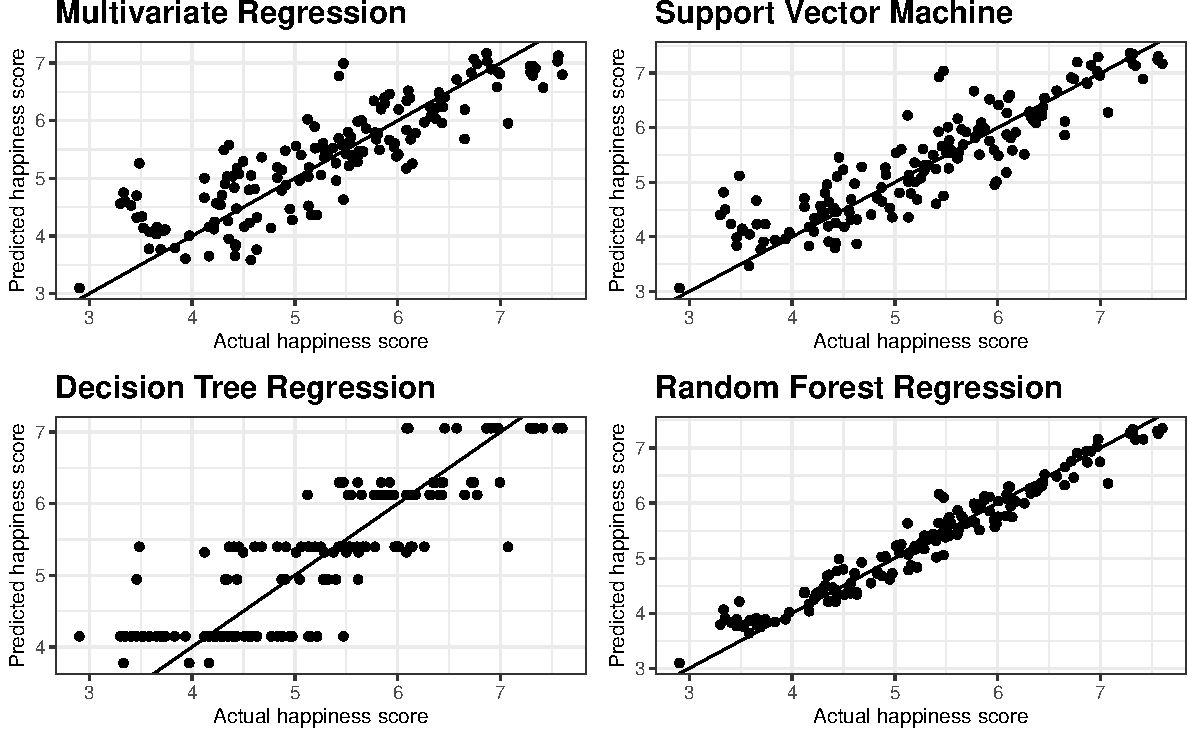
\includegraphics{Assignment4_files/figure-latex/training-1.pdf}
\caption{\label{fig:training}Model Training Split Ratio is 0.8}
\end{figure}

\hypertarget{random-forest-regression}{%
\subsubsection{Random Forest regression}\label{random-forest-regression}}

Random Forest Model has a variable selecting system (via bootstrapping) to decide the most significant tree and is able to reduce overwriting compared to the decision tree. With that said, the random forest is a strong modeling technique and more robust than other methods \autocite{liberman2017}. We can see from the plot that this model has captured the data very well in the past few years based on various training sets (see Figure \ref{fig:ggsp04} to \ref{fig:ggsp07}).

By checking the loading for each variable in the RF model, we get the order of importance in Table \ref{tab:varimp}.

\newpage
\begin{table}

\caption{\label{tab:varimp}Variable importance for Random Forest model}
\centering
\begin{tabular}[t]{l|r}
\hline
  & IncNodePurity\\
\hline
\cellcolor{gray!6}{Economy} & \cellcolor{gray!6}{348.6690}\\
\hline
Health & 327.0846\\
\hline
\cellcolor{gray!6}{Freedom} & \cellcolor{gray!6}{169.3299}\\
\hline
Generosity & 97.7974\\
\hline
\end{tabular}
\end{table}

Based on the result in Table \ref{tab:varimp}, the most important variable is Economy, followed by Health, Freedom and Generosity being the last.

\hypertarget{multivariate-linear-model-analysis.}{%
\subsection{Multivariate Linear Model Analysis.}\label{multivariate-linear-model-analysis.}}

The RF model helps us to determine which variables to choose in the multivariate linear regression model. The advantage of using multivariate linear regression is that it can allow us to analyse the relationship between different variables in a statistical coherent way \autocite{voxco2022},such as, marginal effects and percentage changes.

If using a classic linear model with all four variables,

\[
\begin{aligned}
Happiness\ score=& Economy+Health+Generosity+Freedom
\end{aligned}
\]

They have similar impacts on explaining the happiness score and all of them are significant in Table \ref{tab:without}. Thus, it is hard to tease the importance of each variable out with this model.

\begin{table}

\caption{\label{tab:without}Linear regression model for happiness scores without new data}
\centering
\begin{tabular}[t]{l|r|r|r|r}
\hline
  & Estimate & Std. Error & t value & Pr(>|t|)\\
\hline
\cellcolor{gray!6}{(Intercept)} & \cellcolor{gray!6}{2.4374} & \cellcolor{gray!6}{0.0753} & \cellcolor{gray!6}{32.3704} & \cellcolor{gray!6}{0}\\
\hline
Health & 1.2232 & 0.1392 & 8.7871 & 0\\
\hline
\cellcolor{gray!6}{Economy} & \cellcolor{gray!6}{1.4543} & \cellcolor{gray!6}{0.0842} & \cellcolor{gray!6}{17.2820} & \cellcolor{gray!6}{0}\\
\hline
Freedom & 1.3722 & 0.1096 & 12.5222 & 0\\
\hline
\cellcolor{gray!6}{Generosity} & \cellcolor{gray!6}{1.1702} & \cellcolor{gray!6}{0.1397} & \cellcolor{gray!6}{8.3785} & \cellcolor{gray!6}{0}\\
\hline
\end{tabular}
\end{table}

As a result, we will drop the least insignificant two and add another two new variables, Consumer Price Index and the population size of each country, gained from the World Bank data from 2016 to 2022 \autocite{world2022}. After matching the data for each country and drop the NA values, we can use the new dataset to construct a new Linear model. Nevertheless, due to the lack of data in 2021 and 2022, we can only use the data up to 2020.

\[
\begin{aligned}
\textbf{New Multivariate Linear Model with a natural log of score}:\\
log(score)= -4.6000-0.0008\ cpi+0.2591\ log(economy)\\-0.0026\ log(population)+0.0114\ log(health)+0.0032\ year
\end{aligned}
\]

\begin{table}

\caption{\label{tab:mle}Multivariate Linear regression model for the log data with R-squared is 0.6076}
\centering
\begin{tabular}[t]{l|r|r|r|r}
\hline
  & Estimate & Std. Error & t value & Pr(>|t|)\\
\hline
\cellcolor{gray!6}{(Intercept)} & \cellcolor{gray!6}{-4.5999} & \cellcolor{gray!6}{11.5632} & \cellcolor{gray!6}{-0.3978} & \cellcolor{gray!6}{0.6909}\\
\hline
cpi & -0.0008 & 0.0002 & -4.2994 & 0.0000\\
\hline
\cellcolor{gray!6}{log\_eco} & \cellcolor{gray!6}{0.2591} & \cellcolor{gray!6}{0.0094} & \cellcolor{gray!6}{27.5487} & \cellcolor{gray!6}{0.0000}\\
\hline
log\_population & -0.0026 & 0.0036 & -0.7072 & 0.4797\\
\hline
\cellcolor{gray!6}{log\_health} & \cellcolor{gray!6}{0.0114} & \cellcolor{gray!6}{0.0042} & \cellcolor{gray!6}{2.7419} & \cellcolor{gray!6}{0.0063}\\
\hline
year & 0.0032 & 0.0057 & 0.5508 & 0.5820\\
\hline
\end{tabular}
\end{table}

We can see in Table \ref{tab:mle} that 60.76\% of the variation in \(log(score)\) can be explained by the model. It is noticeable that the economy status(GDP per capita) has the largest influence on the happiness scores than other variables.

Besides, in econometric contexts, coefficients in the log-log model can be interpreted as the percentage change in dependent variable when there is a one percentage change increase in the regressor \autocite{benoit2011}.

For example:

\begin{align*}
\frac{\Delta \text{ log(Happiness Score)}}{\Delta \text{ log(Economy)}} &\approx \frac{\Delta \text{ Happiness Score}}{\Delta \text{ Economy} }\frac{\text{Economy}}{\text{Happiness Score}}\\
&=\frac{\% \Delta \text{ Happiness Score}}{\% \Delta \text{ Economy}} \nonumber\\
&= \text{ME(Coefficient)}\nonumber\\
&= 0.2591
\end{align*}

Here, we can interpret that a 1\% increase in Economy(measured in GDP per capita) will increase the happiness score by 0.2591\%, keeping all other regressors constant. Similarly for the rest variables, a 1\% percent increase in health will increase happiness by 0.0114\%. On the contrary, we can see that an increase in population and CPI have negative impacts, which are -0.0026\% for Population and -0.08 for CPI respectively.

\hypertarget{endogenity-and-sample-selection-bias}{%
\subsection{Endogenity and Sample Selection Bias}\label{endogenity-and-sample-selection-bias}}

This model may have an endogenous problem, which is caused by omitting variables, as we only include 5 relevant variables in the model. There are some latent variables that affect the happiness score but are not included in this model such as education level and culture backgrounds.

\begin{figure}
\centering
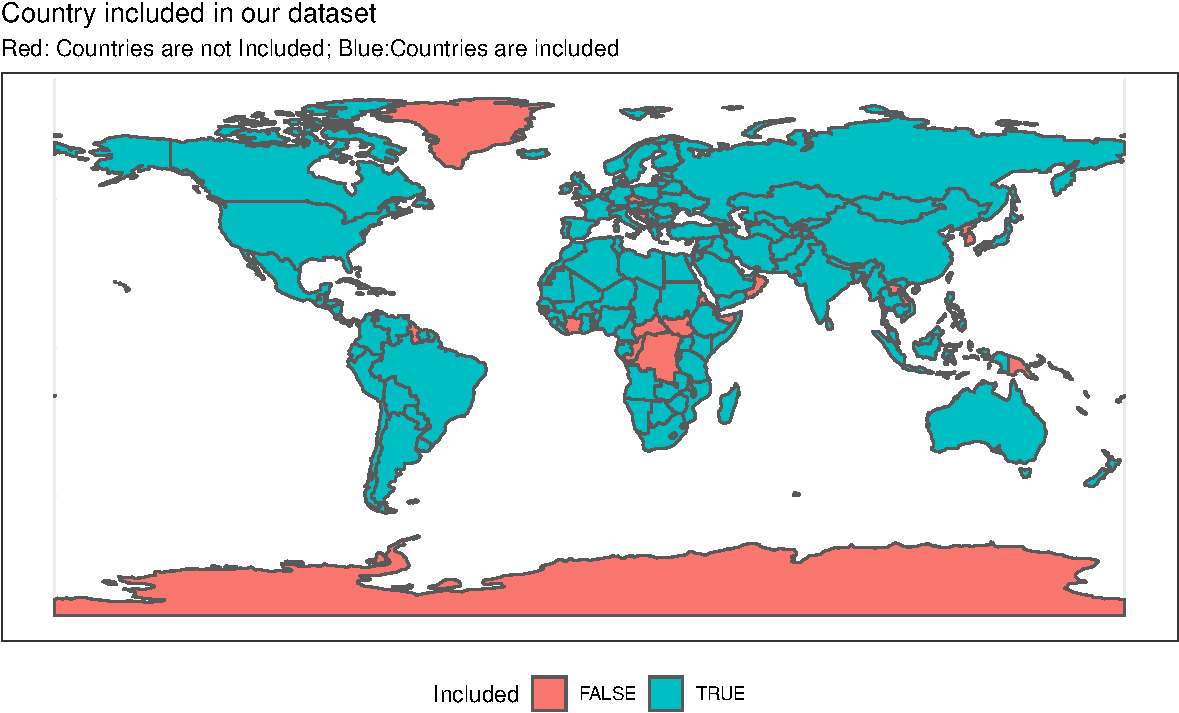
\includegraphics{Assignment4_files/figure-latex/worldmapall-1.pdf}
\caption{\label{fig:worldmapall}Colour the country that have included in Worldmap}
\end{figure}

Apparently, our model also has some bias in sample selection. In our model, data for 34 countries are not included, which are colored in red in Figure \ref{fig:worldmapall}. These missing countries are either sparsely populated or still in development, so the model is not revealing all information due to the sample selection bias. To solve this, sample selection models such as Heckman model or Tobit can be considered in Econometrics areas.

\newpage

\hypertarget{residual-diagonistic-for-the-regression-model}{%
\subsection{Residual Diagonistic for the Regression Model}\label{residual-diagonistic-for-the-regression-model}}

From the Residual and Fitted plot in Figure \ref{fig:resd}, we can see it has a non-constant variance across the fitted value, which indicates the presence of Heteroskedasticity. Moreover, the error distribution (see Figure \ref{fig:density}) and the Q-Q plot Figure (see both Figure \ref{fig:qq} and Figure \ref{fig:inf} also suggest the density of our model is somewhat to a normal distribution but influenced by outliers.

In conclusion, our model did a good job in explaining the relationships between happiness score and our selected aggressors even though there are still some limitations.

\begin{figure}
\centering
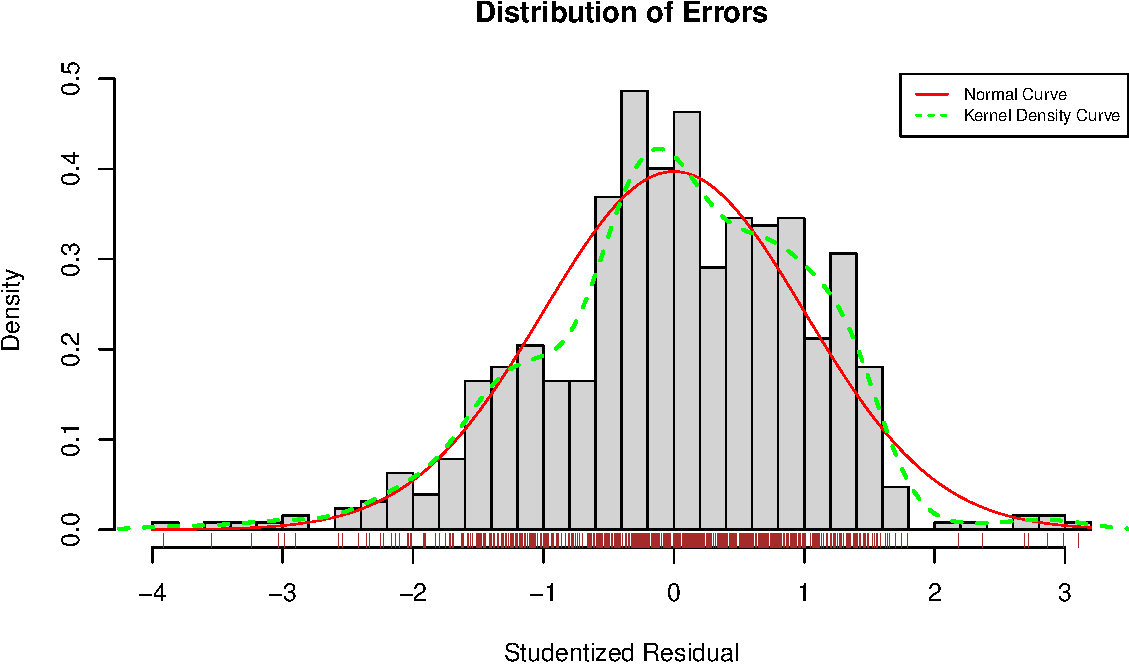
\includegraphics{Assignment4_files/figure-latex/density-1.pdf}
\caption{\label{fig:density}Distribution of the residual term}
\end{figure}

\begin{figure}
\centering
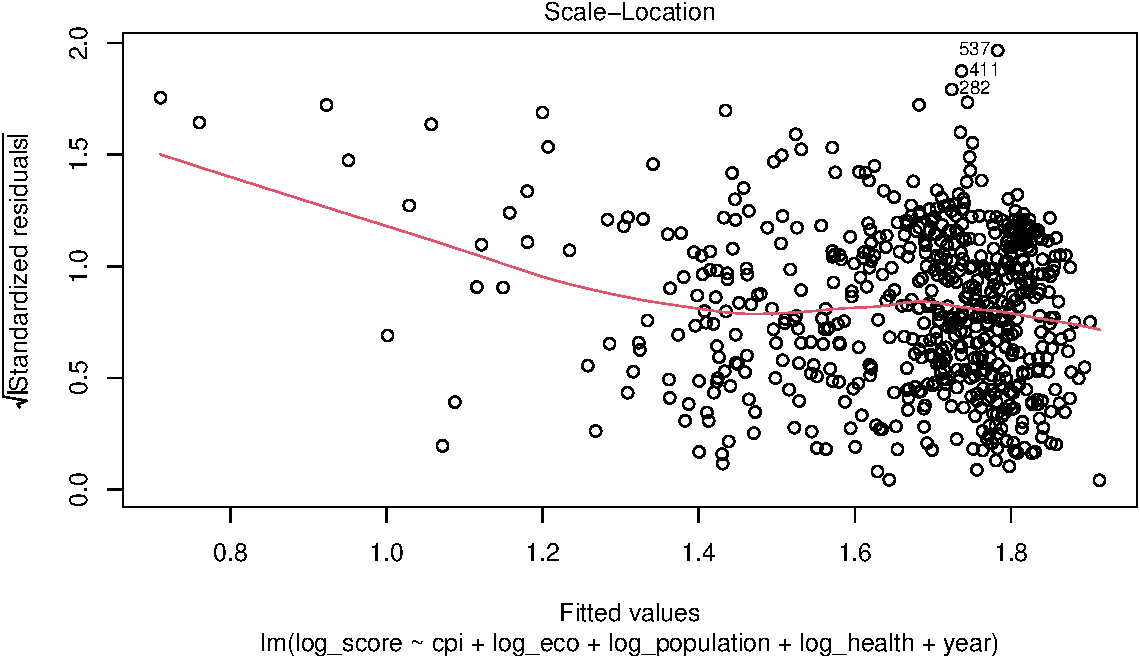
\includegraphics{Assignment4_files/figure-latex/resd-1.pdf}
\caption{\label{fig:resd}Residual vs Fitted value plot (with standardised residuals)}
\end{figure}

\begin{figure}
\centering
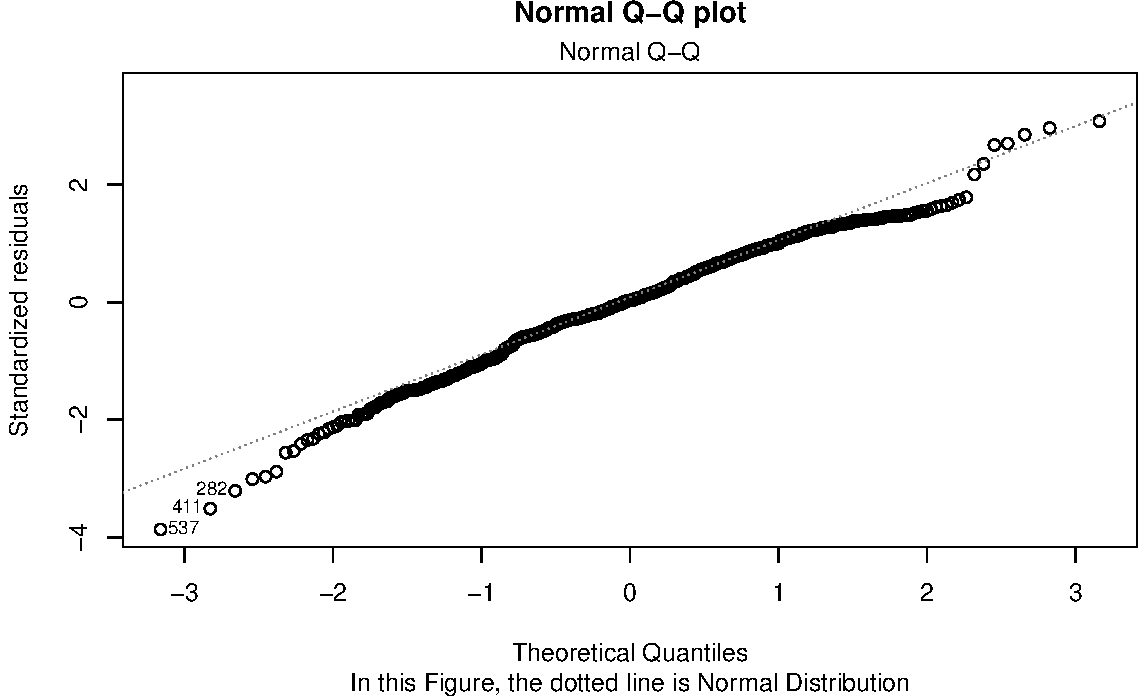
\includegraphics{Assignment4_files/figure-latex/qq-1.pdf}
\caption{\label{fig:qq}Q-Q plot fitted model residual density vs normal distribution residual density}
\end{figure}

\begin{figure}
\centering
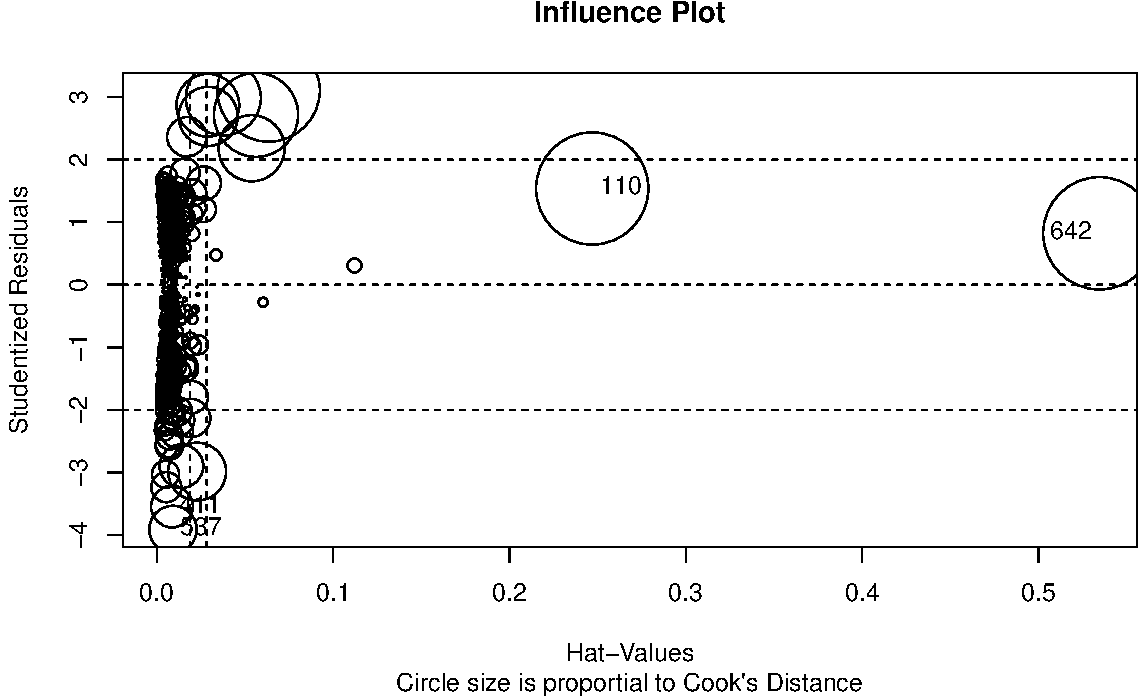
\includegraphics{Assignment4_files/figure-latex/inf-1.pdf}
\caption{\label{fig:inf}Influence Plot, the bigger circle means outliers}
\end{figure}

\clearpage

\hypertarget{conclusion}{%
\section{Conclusion}\label{conclusion}}

According to above the analysis, we can conclude that the Happiness Scores are closely related to the economic activities and health status. In those developed countries with better living and health conditions, people generally feel happier than those people living in rural areas.

On the other hand, we find that the happiness scores for people living in Sub-Saharan and Southeast Asia are relatively low, which is mainly due to the poor economic development and harsh living environment \autocite{helliwell2021world}. In terms of the happiness scores at region level, Europe is the most livable continent with majority of countries higher than the average level. Even during the pandemic period, people in European countries still feel happier than other regions.

Apart from this, it is evident that during the COVID-19 period, Health, Economy and Social Support have a close relationship with the happiness score. The correlation between health and happiness is much stronger than before.

Through modelling, over years from 2015 to 2022, two most important variables in explaining the happiness scores across different countries are Economy (measured in GDP per capita) and Health. Based on the results in the final multivariate linear model, Economy is the most significant and essential factor.

Furthermore, using the advantage of linear model, both Economy and Health status have positive marginal effect on the happiness score, while CPI and Population have negative impacts.

Nevertheless, we still need to deal with the presence of heteroskedasticity, the endogeneity bias and possible sample selection bias to improve the accuracy and usefulness of our model. Further studies can be done to minimizing these limitations and come up with a better modelling for global macroeconomic data.

\hypertarget{acknowledgement}{%
\section{Acknowledgement}\label{acknowledgement}}

We shall never forget the hard works done by our lecturer \textbf{Patricia} on every Tuesday nights from Week 1 to Week 12.

We will also remember our tutors \textbf{Naveen} and \textbf{Fan}. They performed hard works on our tutorials and gave us nice recommendations during the presentation session.

Moreover, we'd like to thank all \textbf{EBS scholars} from \textbf{Monash University} for their excellent \texttt{monash} package produced such a nice report template.

Without any of their help, our works could not get finished so smoothly.

Overall, I'd also like to thank those package developers who fight for the open source software, which made us easier to plot so many beautiful plots.

Here are the lists of packages we used:

\begin{itemize}
\tightlist
\item
  package tidyverse \autocite{tidyverse}
\item
  package GGally \autocite{GGally}
\item
  package ggplot2 \autocite{ggplot2}
\item
  package readr \autocite{readr}
\item
  package dplyr \autocite{dplyr}
\item
  package gridExtra \autocite{gridExtra}
\item
  package RColorBrewer \autocite{RColorBrewer}
\item
  package gganimate \autocite{gganimate}
\item
  package repr \autocite{repr}
\item
  package neuralnet \autocite{neuralnet}
\item
  package ggpubr \autocite{ggpubr}
\item
  package caTools \autocite{caTools}
\item
  package rworldmap \autocite{rworldmap}
\item
  package rnaturalearth \autocite{rnaturalearth}
\item
  package sf \autocite{sf}
\item
  package car \autocite{car}
\item
  package kableExtra \autocite{kableExtra}
\item
  package here \autocite{here}
\item
  package lubridate {[}lubridate{]}
\item
  package cowplot \autocite{cowplot}
\item
  package janitor \autocite{janitor}
\item
  package maps \autocite{maps}
\item
  package plotly \autocite{plotly}
\item
  package wbstats \autocite{wbstats}
\item
  package lemon \autocite{lemon}
\item
  package sp \autocite{sp}
\end{itemize}

\clearpage

\hypertarget{appendix}{%
\section{Appendix}\label{appendix}}

\begin{align*}
\intertext{We here take the Economy Situation (measured in GDP per capita) as an example:}
\frac{\partial \text{log(Happiness Score)}}{\partial \text{log(Economy)}} &= \text{ME(Coefficient)}\\
\intertext{From (1) we can say, when other variables remain constant }\nonumber \\
\Delta \text{ log(Happiness Score)} &= \text{ME(Coefficient)} \times \Delta \text{ log(Economy)}\\
\intertext{By using the infinite approaching approximation of log function, we can know}\nonumber\\
log(x_0 + \Delta x) - log(x_0) &\approx log(x_0) + log'(x_0)\Delta x - log(x_0)\\
&=  \frac{\Delta x}{x_0} = \text{percentage change in x}\nonumber\\
\intertext{Therefore}\nonumber\\
\frac{\Delta \text{ log(Happiness Score)}}{\Delta \text{ log(Economy)}} &\approx \frac{\Delta \text{ Happiness Score}}{\Delta \text{ Economy} }\frac{\text{Economy}}{\text{Happiness Score}}\\
&=\frac{\% \Delta \text{ Happiness Score}}{\% \Delta \text{ Economy}} \nonumber\\
&= \text{ME(Coefficient)}\nonumber
\end{align*}

\begin{figure}

{\centering 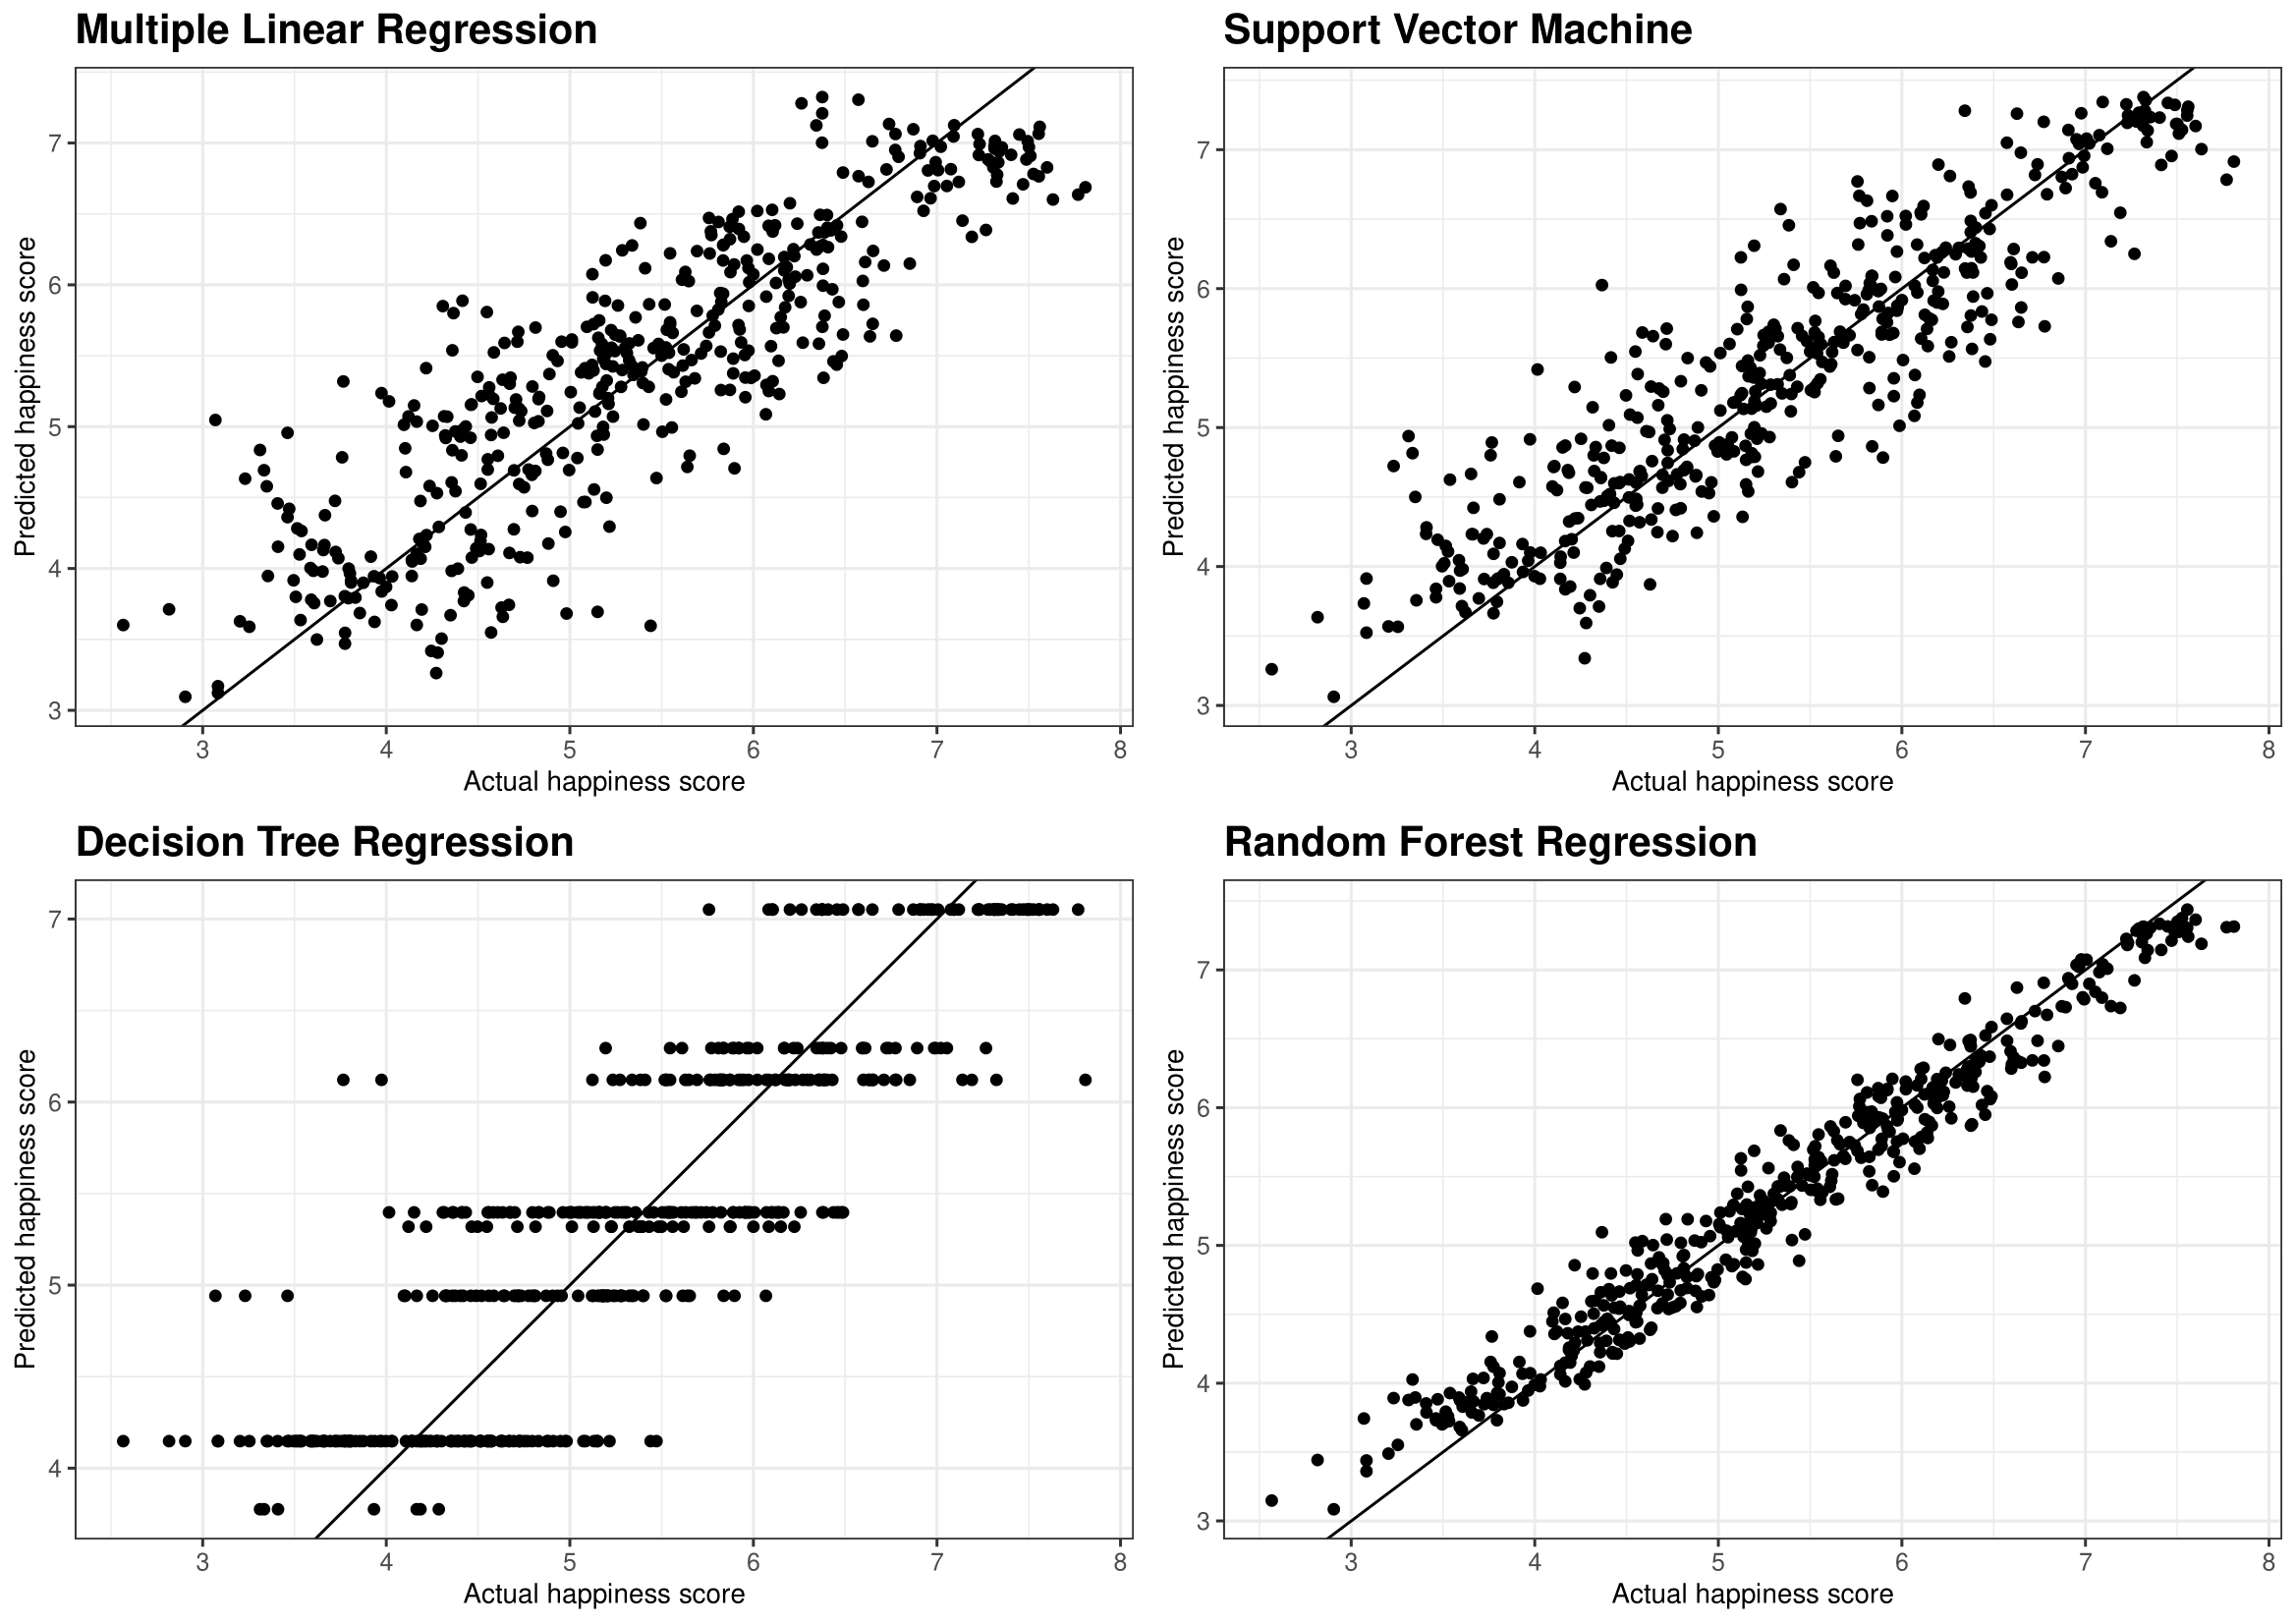
\includegraphics[width=0.7\linewidth]{figure/ggsp04} 

}

\caption{Models' performance under the training test split ratio = 0.4}\label{fig:ggsp04}
\end{figure}

\begin{figure}

{\centering 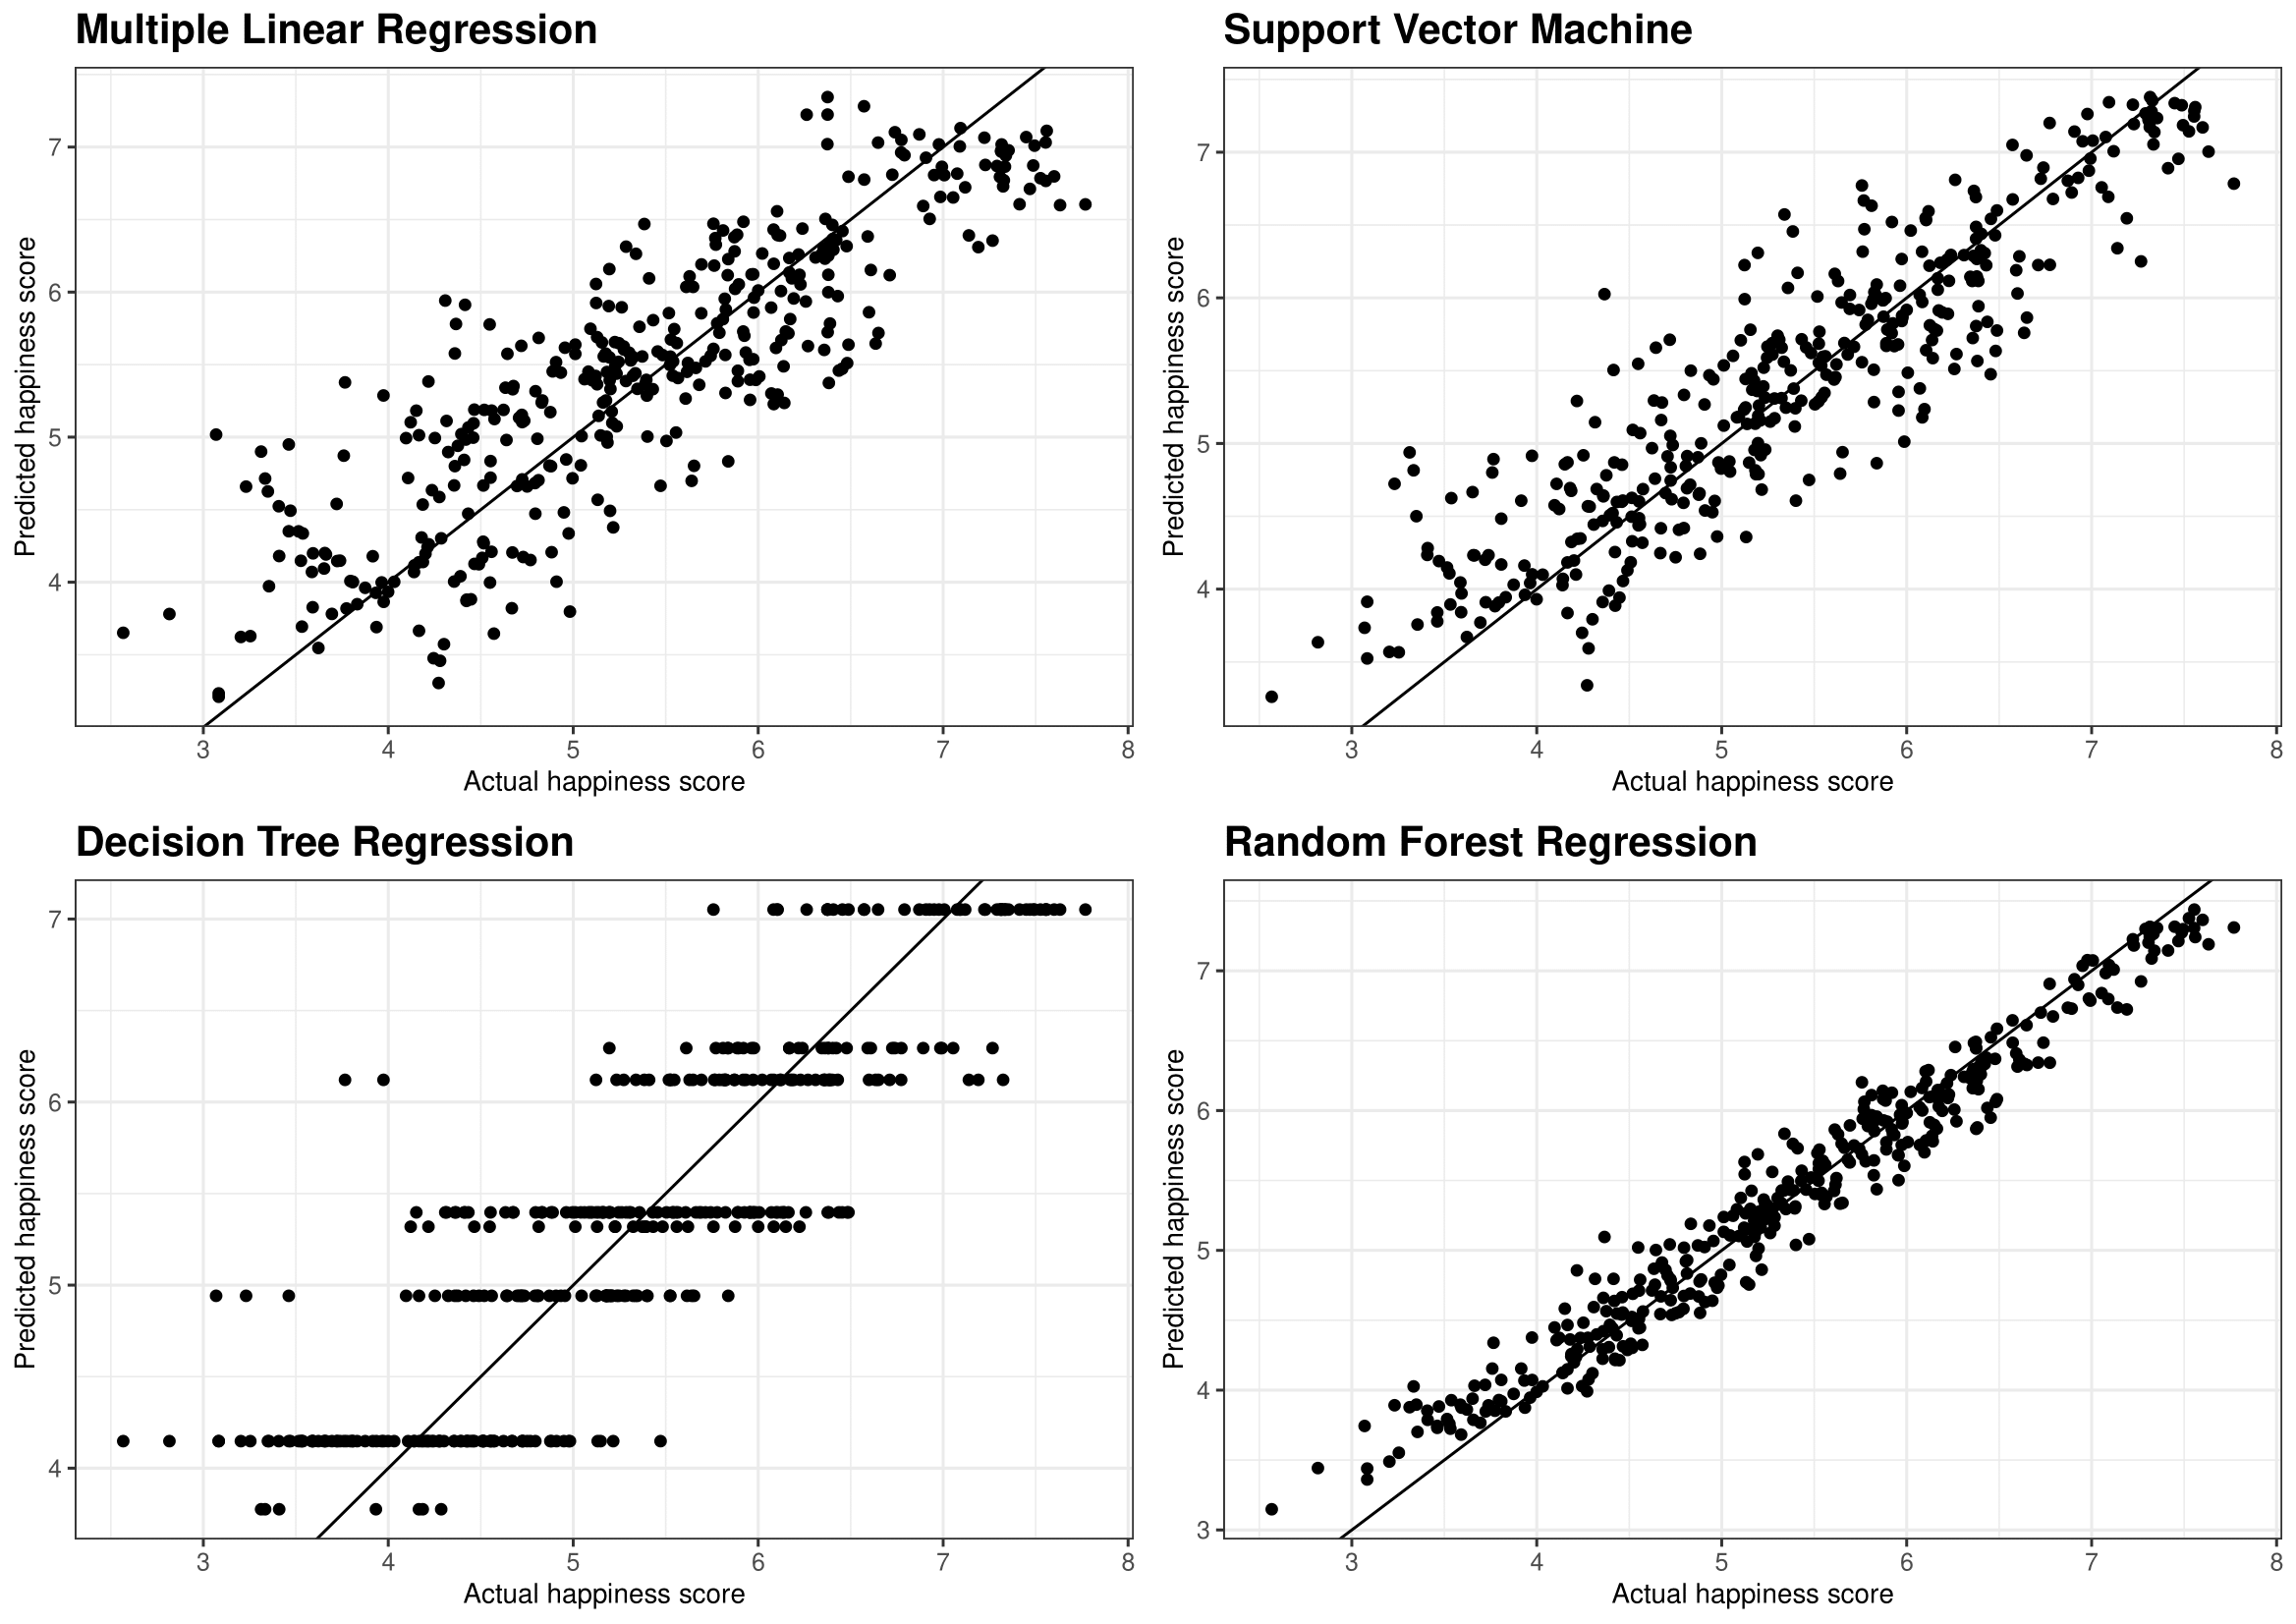
\includegraphics[width=0.7\linewidth]{figure/ggsp05} 

}

\caption{Models' performance under the training test split ratio = 0.5}\label{fig:ggsp05}
\end{figure}

\begin{figure}

{\centering 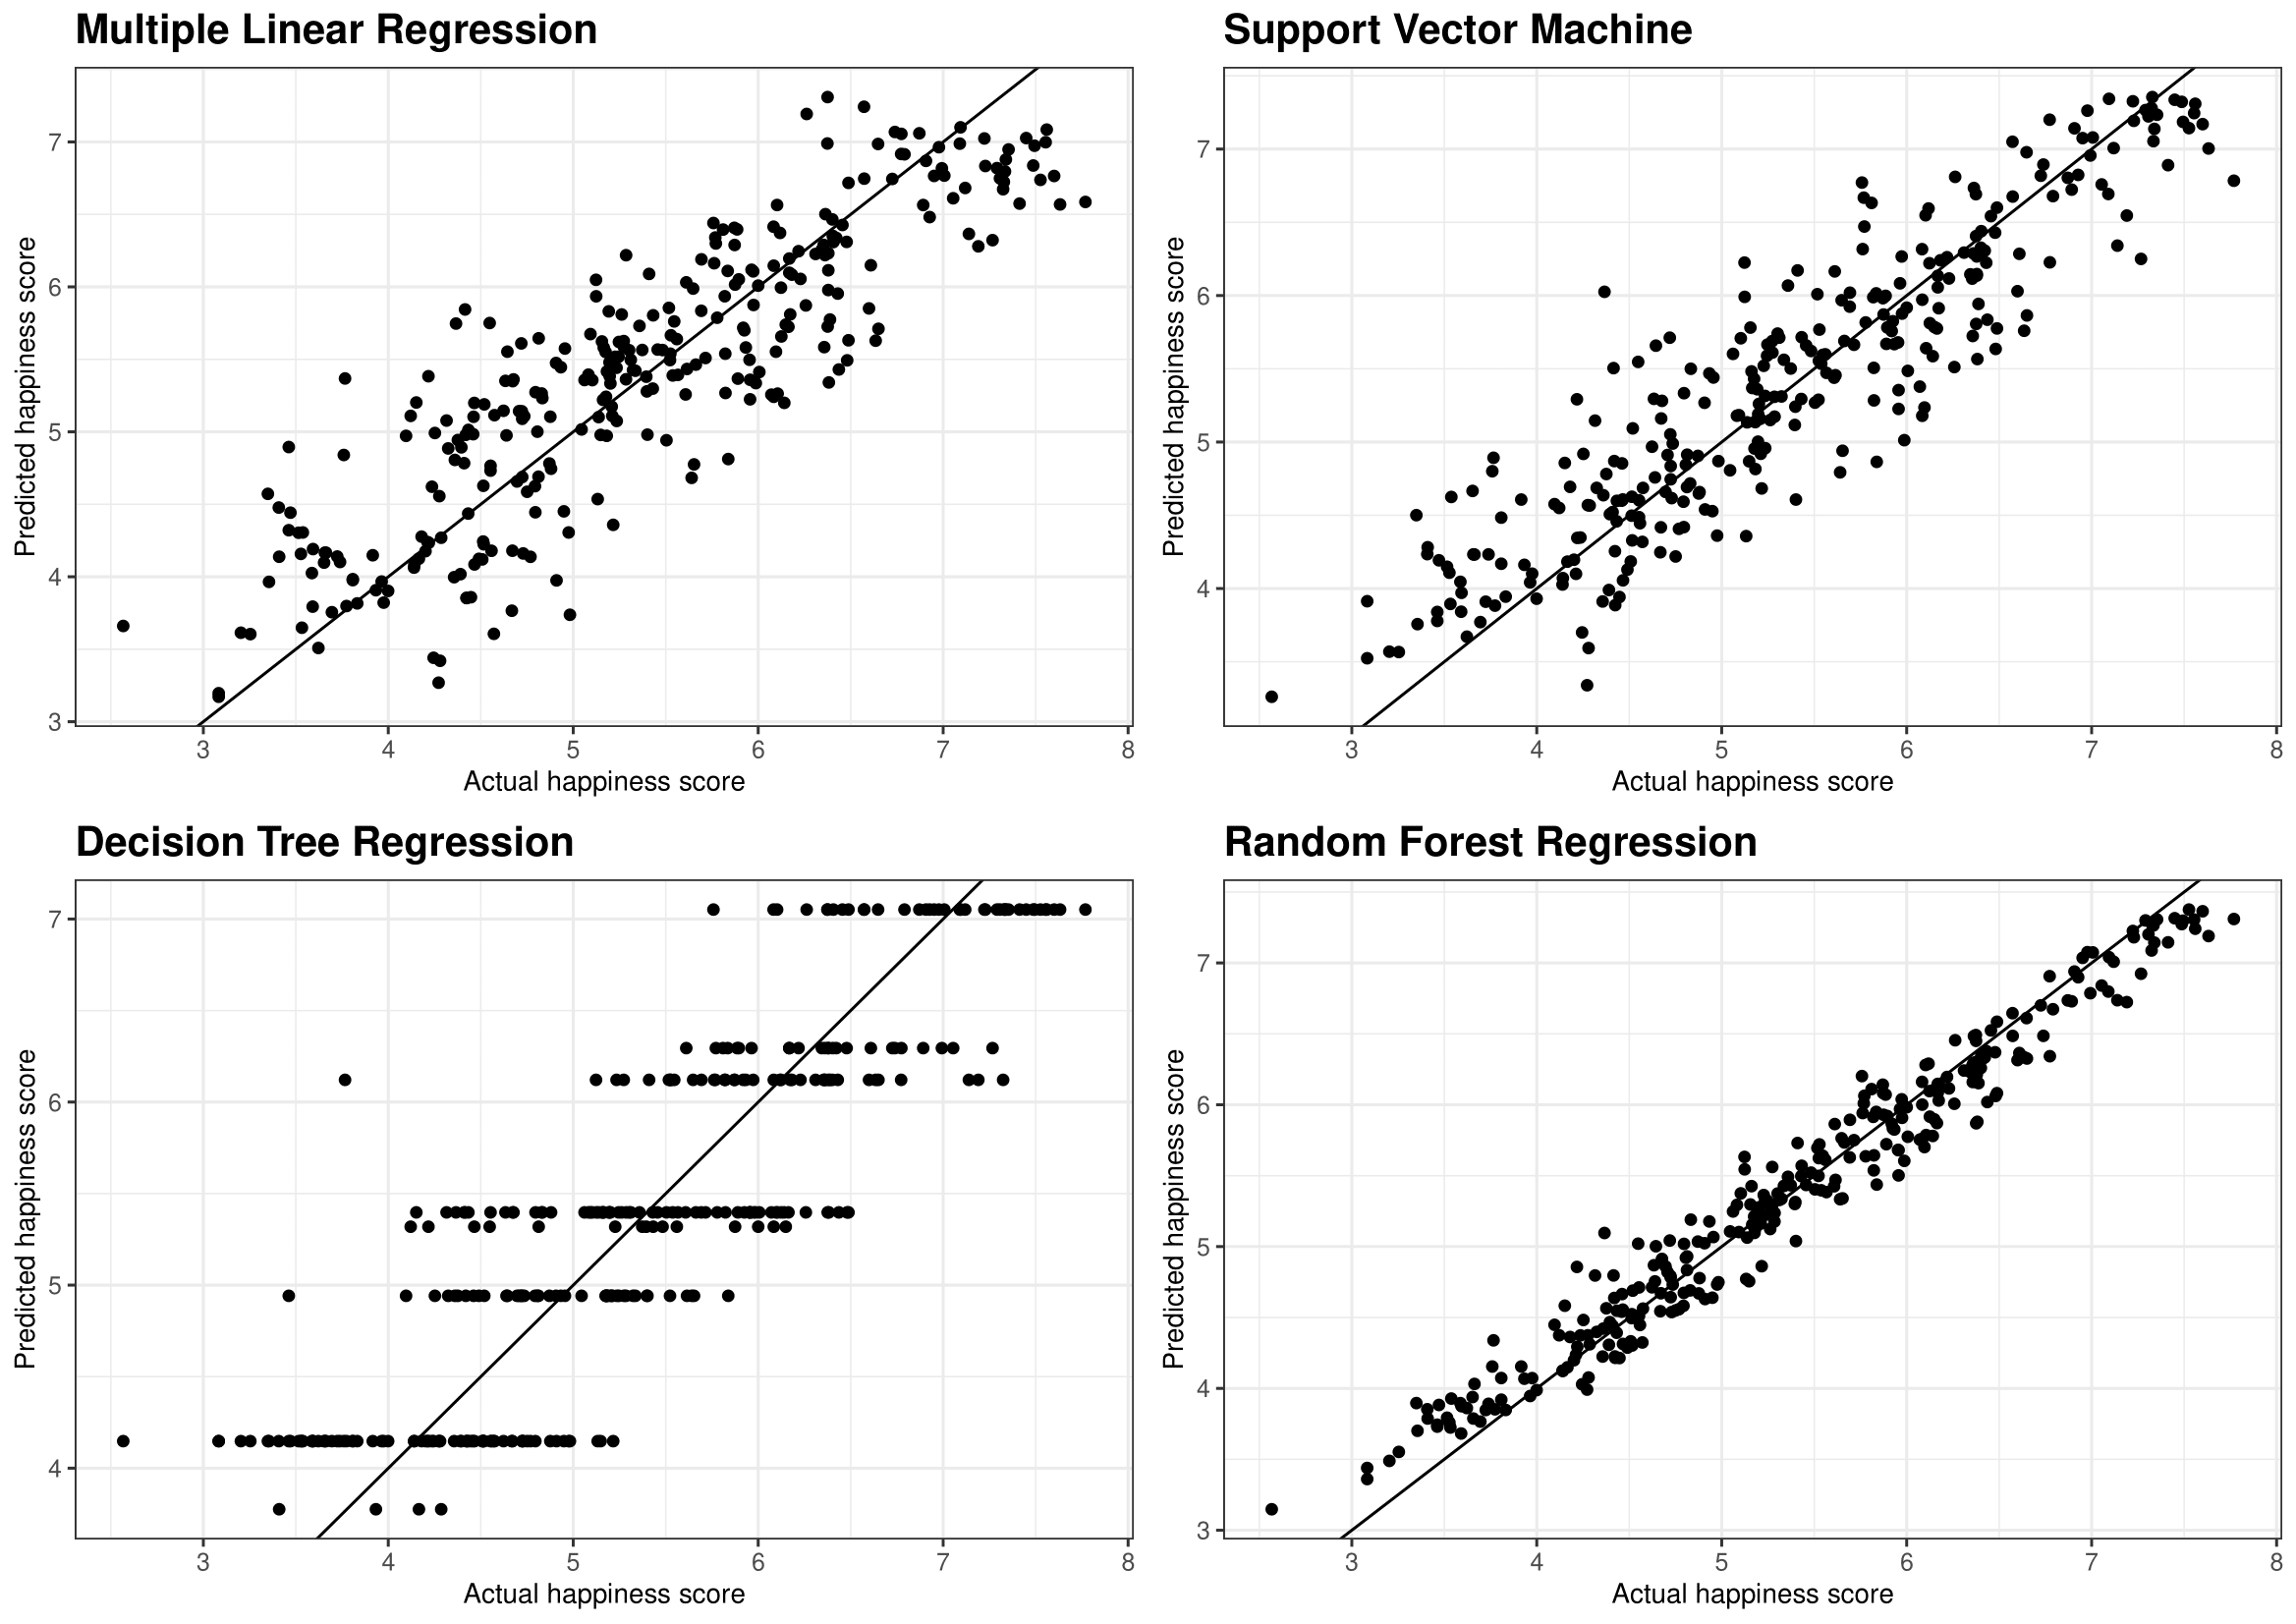
\includegraphics[width=0.7\linewidth]{figure/ggsp06} 

}

\caption{Models' performance under the training test split ratio = 0.6}\label{fig:ggsp06}
\end{figure}

\begin{figure}

{\centering 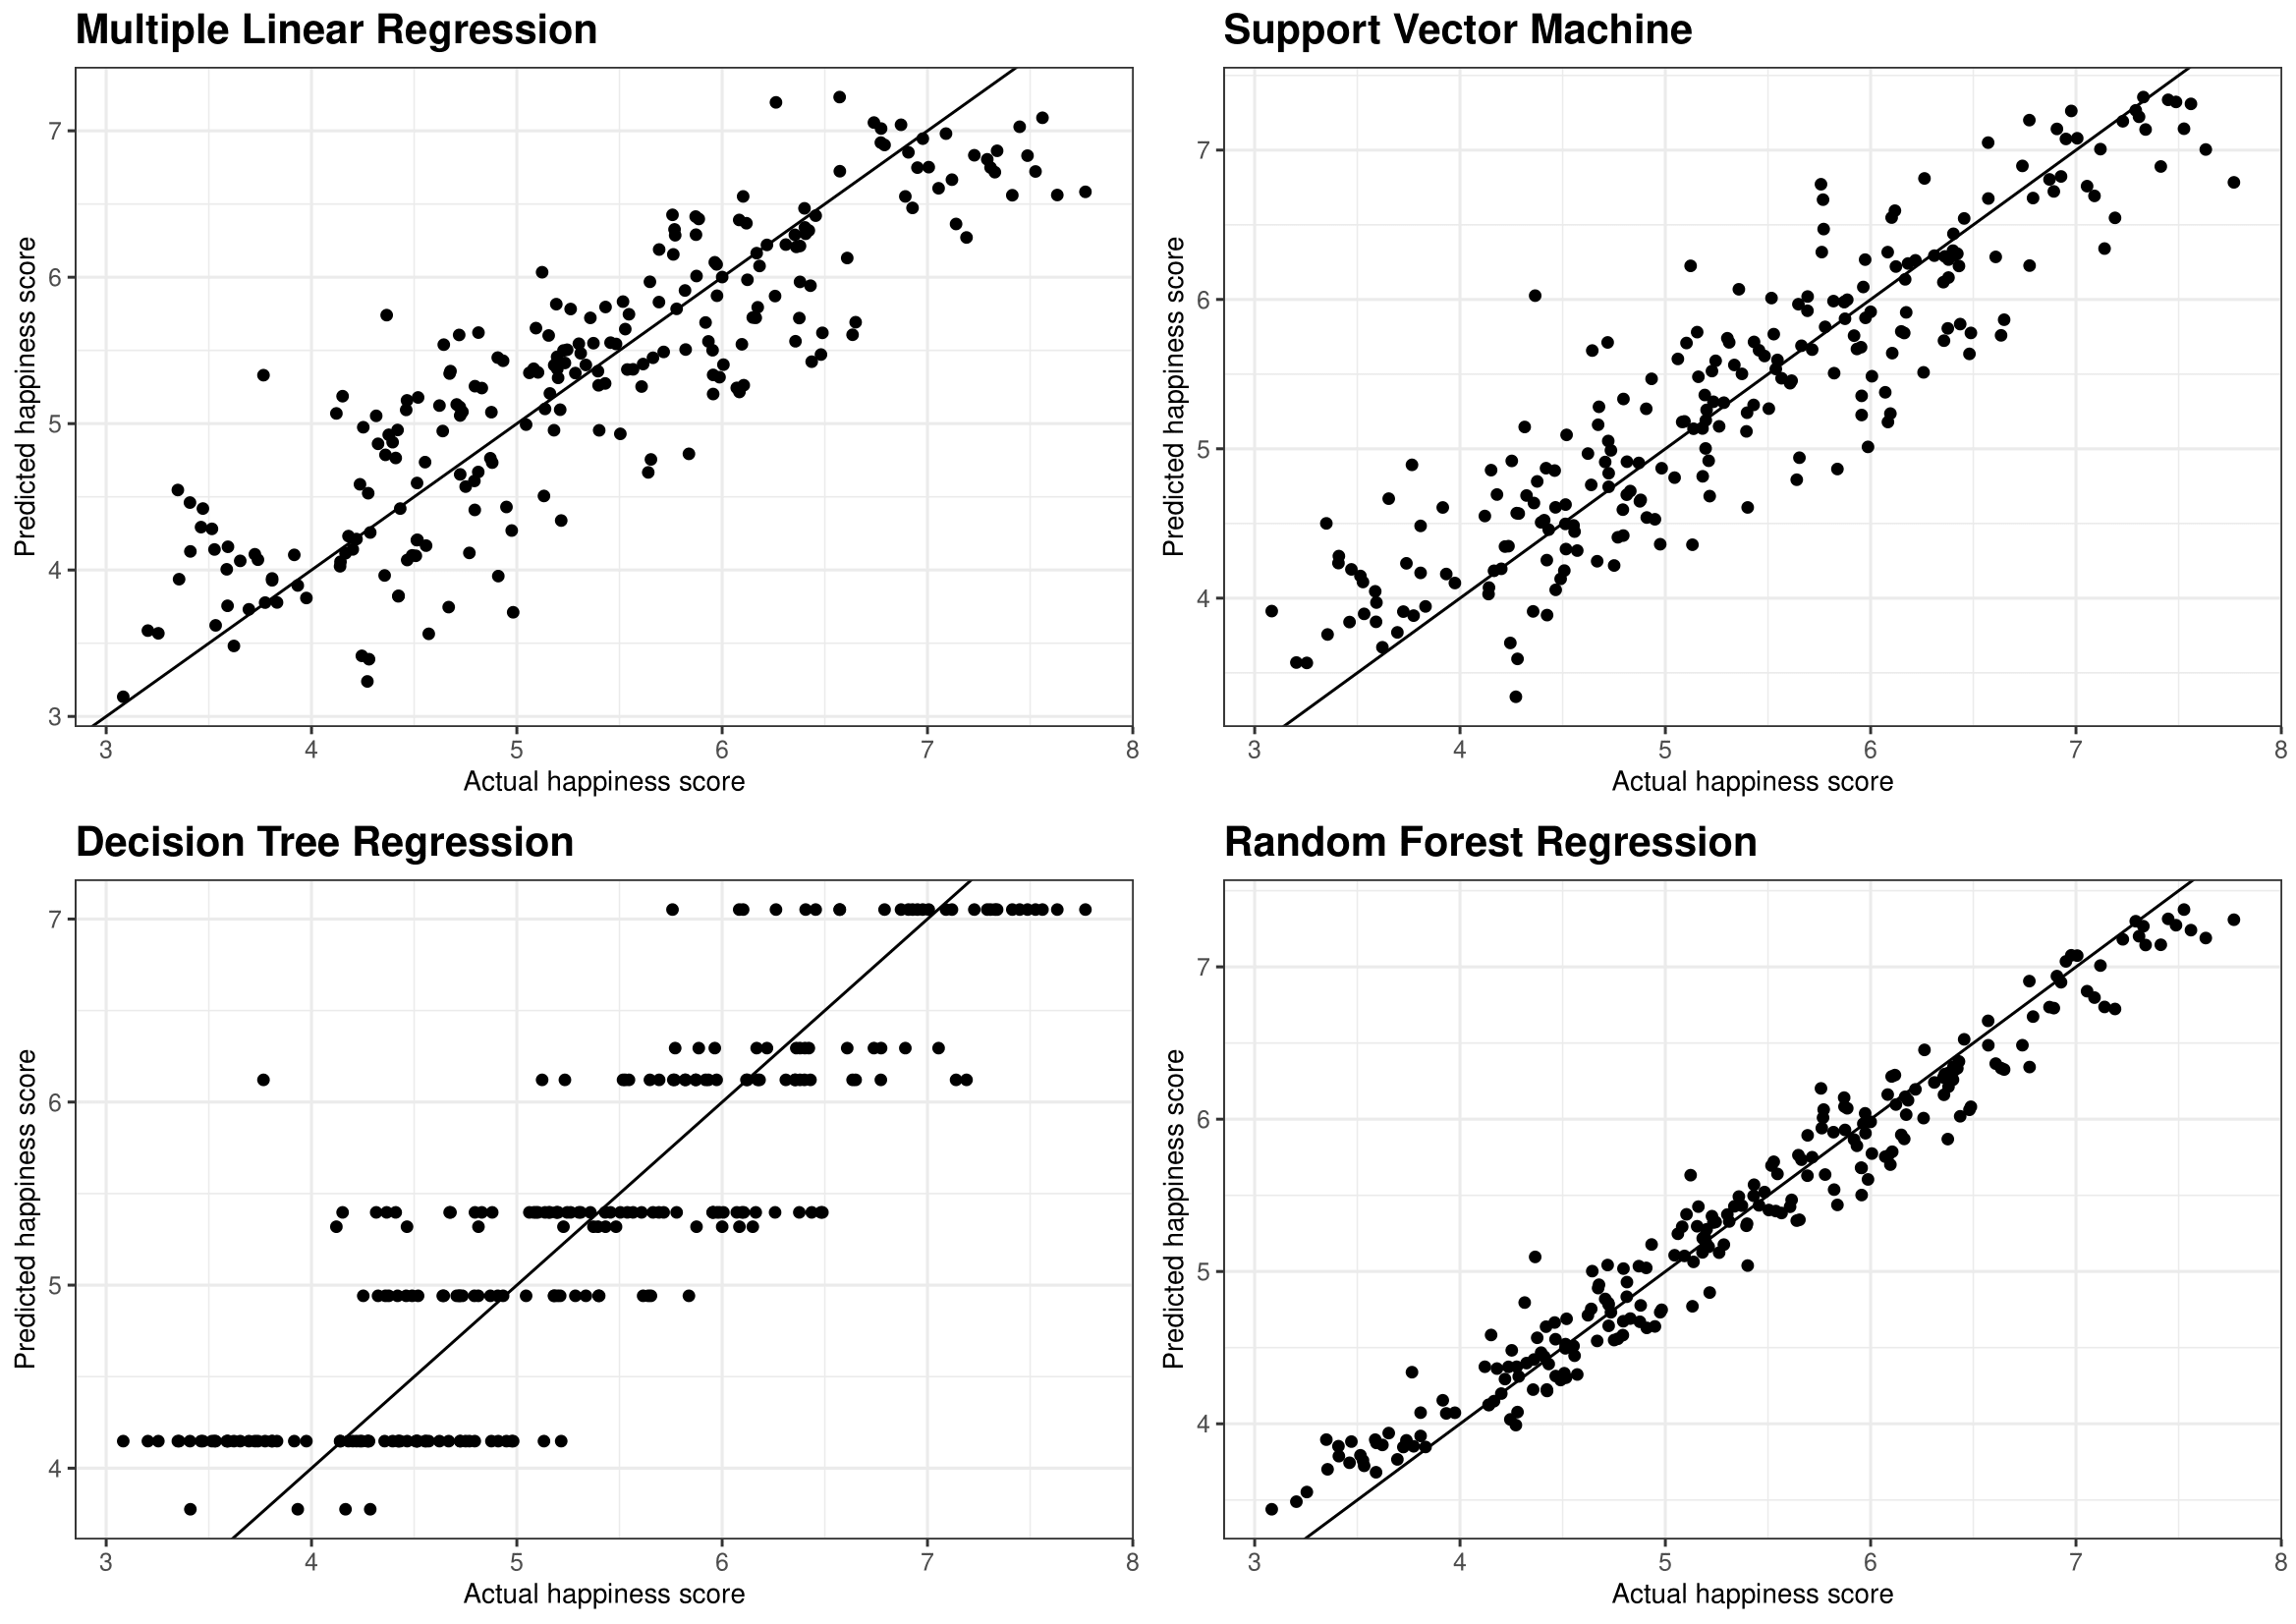
\includegraphics[width=0.7\linewidth]{figure/ggsp07} 

}

\caption{Models' performance under the training test split ratio = 0.7}\label{fig:ggsp07}
\end{figure}

\clearpage

\printbibliography

\end{document}
